
% pgf settings: shrink the tick labels a bit
\pgfplotsset{every tick label/.append style={font=\scriptsize}}

\newcommand{\scatterplotsize}{8cm}
\newcommand{\scatterplotxlabelshift}{1.5ex}
\newcommand{\scatterplotylabelshift}{-3ex}



\section{Experiments}
\label{experiments}

%% \joerg{1.5--2 page: similar to ijcai version; expliucotly distinguish 
%% global vs local, add results for local in both ipc and action-set prop
%% experiments}

We implemented our approach in Fast Downward
(FD) \cite{helmert:jair-06}. We evaluate it, in turn, on IPC
benchmarks modified for OSP planning, and on a selection of IPC
benchmarks we extended with action-set properties.

The base planner called by our SysS and SysW algorithms on each search
node runs forward search using
\hff\ \cite{hoffmann:nebel:jair-01}, optionally with conjunction or trap learning.
%
%% The base planner configurations, used to solve/prove unsolvability
%% of a meta search node, are greedy best first search with $\hff$ and
%% preferred operators ($hff$) and conjunction learning $\hc$ with
%% $\hff$ as its base heuristic. \rebecca{ask Marcel how it is
%% called} \rebecca{Modification of hC to find deadends with an cost
%% bound}
%
The experiments were run on a cluster of Intel E5-2660 machines
running at 2.20 GHz, with time (memory) cut-offs of 30 minutes (4 GB).



 



%%%%%%%%%%%%%%%%%%%%%%%%%%%%%%%%%%%%%%%%%%%%%%%%%%%%%%%%%%%%%%%%%%%%
%%%%%%%%%%%%%%%%%%%%%%%%%%%%%%%%%%%%%%%%%%%%%%%%%%%%%%%%%%%%%%%%%%%%
%%%%%%%%%%%%%%%%%%%%%%%%%%%%%%%%%%%%%%%%%%%%%%%%%%%%%%%%%%%%%%%%%%%%
%%%% IPC OSP

\subsection{IPC-Based OSP Benchmarks}
\label{experiments:ipc}

% The net-benefit benchmarks don't give us anything new (the ones we
% could use are adopted from IPC ben chmarks anyhow).
%
%% \joerg{Rebecca/Michael: check out the IPC net-benefit benchmarks. Reviewers may naturally expect us to experiment with those, given our strong focus on oversubscription planning (actually this question came up in the discussion with the NASA guys yesterday). In the net-bnefit benchmarks, goal facts have rewards which we don't need. The question is whether, stripping away these rewards and imposing a plan-cost bound, we would get benchmarks not already covered by bour IPC experiments anyway. If the answer is "no", we can just say so in the paper. If the answer is "yes", it would be good (though probably not absolitely necessary) to experiment with these domains as well. In any case, we should know what the answer is.}

Following Katz et al.\ \shortcite{katz:etal:icaps-19}, for every IPC
benchmark task $(\vars,\acts,\cost,\init,\goal)$ with smallest known
plan cost $C$ as per planning.domains \cite{muise:icaps-demos-16}, we
obtained three OSP tasks by setting the cost bound to $b = x * C$
where $x \in \{0.25, 0.5, 0.75\}$. We used soft goals only, \ie,
$\goalsoft = \goal$ and $\goalhard=\emptyset$. For implementation
reasons, we omitted tasks with $\geq 32$ goals (which would be
infeasible for MUGS analysis anyhow).
%
%% ; the latter is an artifact of our current implementation that
%% could be overcome in principle, though computing all MUGS for that
%% many goals is presumably typically infeasible anyway.
%
% Joerg: said up front where it belongs
%
%% We extended conjunction learning \cite{steinmetz:hoffmann:ai-17} to
%% deal with cost bounds, thus enabling nogood learning and transfer in
%% SysS and SysW.
%
We consider conjunction learning, but not trap learning as that cannot
deal with OSP cost bounds.
%
%% In what follows, we consider first global explanations, then discuss
%% how the picture changes for local explanations.


\subsubsection{IPC Global Explanations}

\setlength{\tabcolsep}{2pt}
\renewcommand{\arraystretch}{0.8}
\begin{figure*}[h!]
\tiny
%\centering 	\tiny
	\begin{tabular}{l|rrr|rrr|rrr||rrr|rrr|rrr||rrr|rrr|rrr}
		& \multicolumn{9}{c||}{0.25} & \multicolumn{9}{c||}{0.5} & \multicolumn{9}{c}{0.75}\\
		& \multicolumn{3}{c|}{coverage} & \multicolumn{3}{c|}{avg time} & & & & \multicolumn{3}{c|}{covergae} & \multicolumn{3}{c|}{avg time} & & & & \multicolumn{3}{c|}{coverage} & \multicolumn{3}{c|}{avg time} & & &\\\hline
		& C & C nr & max & C & C nr & max & \#gs & \#n & fn & C & C nr & max & C & C nr & max & \#gs & \#n & fn & C & C nr & max & C & C nr & max & \#gs & \#n & fn\\\hline
		airport (28) & 0.93 & 0.93 & 0.86 & 0.0179 & 0.0296 & 15.5606 & 2.4 & 8.7 & 0.76 & 0.71 & 0.75 & 0.68 & 8.1089 & 3.8531 & 2.5639 & 1.9 & 4.4 & 0.71 & 0.57 & 0.57 & 0.68 & 3.4586 & 2.4734 & 0.256 & 1.0 & 2.4 & 0.61\\
		barman (4) & 1.00 & 1.00 & 1.00 & 0.003 & 0.0075 & 0.0382 & 3.0 & 7.0 & 0.88 & 1.00 & 1.00 & 1.00 & 42.121 & 26.4318 & 4.7071 & 3.0 & 7.0 & 0.88 & 0.00 & 0.00 & 1.00 & - & - & - & - & - & -\\
		blocks (28) & 1.00 & 0.93 & 0.96 & 0.0003 & 0.0006 & 0.0045 & 6.2 & 391.6 & 0.96 & 0.96 & 0.93 & 0.75 & 0.0006 & 0.0022 & 0.2815 & 6.6 & 138.7 & 0.93 & 0.89 & 0.86 & 0.61 & 0.0037 & 0.0072 & 0.7265 & 6.1 & 50.9 & 0.72\\
		data-net (12) & 0.00 & 0.00 & 1.00 & - & - & - & - & - & - & 0.00 & 0.00 & 1.00 & - & - & - & - & - & - & 0.00 & 0.00 & 1.00 & - & - & - & - & - & -\\
		depot (7) & 1.00 & 1.00 & 1.00 & 0.001 & 0.0027 & 0.065 & 4.0 & 36.1 & 0.94 & 1.00 & 1.00 & 1.00 & 1.2503 & 0.325 & 5.7004 & 7.0 & 34.6 & 0.91 & 0.43 & 0.43 & 0.57 & 4.9737 & 0.767 & 3.0968 & 2.7 & 11.0 & 0.68\\
		driverlog (13) & 1.00 & 1.00 & 1.00 & 0.0002 & 0.0007 & 0.0221 & 7.0 & 553.9 & 0.98 & 0.85 & 0.92 & 0.77 & 0.0062 & 0.0167 & 0.1872 & 13.4 & 387.4 & 0.86 & 0.69 & 0.69 & 0.62 & 2.4397 & 0.8843 & 4.7626 & 7.9 & 189.8 & 0.49\\
		elevators (40) & 0.00 & 0.00 & 1.00 &  &  &  &  &  &  & 0.00 & 0.00 & 1.00 & - & - & - & - & - & - & 0.00 & 0.00 & 0.83 & - & - & - & - & - & -\\
		floortile (13) & 0.54 & 0.46 & 0.46 & 0.0027 & 0.0077 & 0.0846 & 88.7 & 2881.7 & 0.99 & 0.15 & 0.15 & 0.15 & 0.4098 & 0.0973 & 0.3864 & 66.0 & 407.5 & 0.80 & 0.08 & 0.15 & 0.15 & 10.6455 & 2.4284 & 1.6908 & 30.0 & 142.0 & 0.28\\
		freecell (15) & 1.00 & 1.00 & 1.00 & 0.0007 & 0.004 & 0.1086 & 4.0 & 15.0 & 0.94 & 1.00 & 1.00 & 1.00 & 2.1944 & 0.3569 & 6.5571 & 4.7 & 15.0 & 0.94 & 0.87 & 0.87 & 0.93 & 3.5732 & 0.7317 & 24.2341 & 3.3 & 12.2 & 0.76\\
		ged (15) & 0.00 & 0.00 & 0.67 & - & - & - & - & - & - & 0.00 & 0.00 & 0.67 & - & - & - & - & - & - & 0.00 & 0.00 & 0.67 & - & - & - & - & - & -\\
		grid (2) & 1.00 & 1.00 & 1.00 & 0.0057 & 0.0068 & 0.0158 & 1.5 & 4.0 & 0.69 & 1.00 & 1.00 & 1.00 & 0.0131 & 0.0162 & 0.7963 & 1.5 & 4.0 & 0.69 & 1.00 & 1.00 & 1.00 & 0.1839 & 0.38 & 30.1363 & 1.0 & 3.0 & 0.56\\
		gripper (7) & 0.71 & 0.71 & 0.71 & 0.0036 & 0.0031 & 0.0089 & 77.4 & 1085.8 & 0.98 & 0.43 & 0.57 & 0.57 & 0.0547 & 0.0164 & 0.0076 & 32.0 & 97.0 & 0.89 & 0.43 & 0.43 & 0.71 & 0.7262 & 0.4556 & 0.0172 & 12.7 & 42.0 & 0.46\\
		hiking (9) & 1.00 & 1.00 & 1.00 & 0.0078 & 0.0079 & 0.1617 & 1.4 & 1.9 & 0.61 & 1.00 & 1.00 & 1.00 & 10.1549 & 4.5974 & 2.5455 & 1.4 & 1.9 & 0.61 & 1.00 & 1.00 & 1.00 & 173.4486 & 105.979 & 3.7597 & 1.0 & 1.9 & 0.61\\
		logistics (26) & 1.00 & 1.00 & 0.85 & 0.0006 & 0.0018 & 2.5104 & 4.6 & 108.1 & 0.95 & 0.77 & 0.85 & 0.58 & 0.0732 & 0.0309 & 2.7788 & 4.6 & 47.2 & 0.84 & 0.54 & 0.58 & 0.46 & 0.2428 & 0.0851 & 0.1558 & 2.2 & 20.5 & 0.63\\
		miconic (141) & 0.45 & 0.46 & 0.40 & 0.0022 & 0.0033 & 0.0261 & 27.9 & 436.3 & 0.91 & 0.28 & 0.35 & 0.32 & 0.0778 & 0.0119 & 0.0405 & 16.3 & 55.2 & 0.82 & 0.25 & 0.28 & 0.32 & 0.5958 & 0.0925 & 0.0495 & 5.5 & 18.7 & 0.61\\
		movie (30) & 1.00 & 1.00 & 1.00 & 0.0001 & 0.0001 & 0.0001 & 7.0 & 127.0 & 0.99 & 1.00 & 1.00 & 1.00 & 0.0008 & 0.0011 & 0.0003 & 35.0 & 120.0 & 0.94 & 1.00 & 1.00 & 1.00 & 0.0086 & 0.0114 & 0.0013 & 21.0 & 64.0 & 0.50\\
		mprime (22) & 1.00 & 1.00 & 1.00 & 0.0076 & 0.0081 & 0.0206 & 1.3 & 1.7 & 0.59 & 1.00 & 1.00 & 1.00 & 0.0079 & 0.009 & 0.354 & 1.2 & 1.7 & 0.59 & 1.00 & 1.00 & 1.00 & 0.0188 & 0.0235 & 13.4521 & 1.2 & 1.7 & 0.59\\
		mystery (17) & 1.00 & 1.00 & 1.00 & 0.0068 & 0.0083 & 0.039 & 1.4 & 2.2 & 0.63 & 1.00 & 1.00 & 1.00 & 0.0076 & 0.0111 & 1.7946 & 1.4 & 2.2 & 0.63 & 1.00 & 1.00 & 0.88 & 0.0085 & 0.0141 & 1.6148 & 1.2 & 2.2 & 0.63\\
		nomystery (14) & 1.00 & 1.00 & 1.00 & 0.0007 & 0.0032 & 0.062 & 7.3 & 144.1 & 0.96 & 0.86 & 0.86 & 0.71 & 0.1669 & 0.0289 & 1.9467 & 12.8 & 46.0 & 0.92 & 0.57 & 0.57 & 0.57 & 1.9144 & 0.363 & 2.3241 & 5.8 & 17.8 & 0.61\\
		openstacks (47) & 0.15 & 0.15 & 0.51 & 0.0011 & 0.0112 & 0.0709 & 6.4 & 314.4 & 0.98 & 0.11 & 0.11 & 0.47 & 0.0087 & 0.0179 & 0.0091 & 4.6 & 30.8 & 0.96 & 0.11 & 0.11 & 0.43 & 0.4592 & 0.4069 & 0.0198 & 5.2 & 29.2 & 0.91\\
		organic-syn (7) & 1.00 & 0.86 & 0.86 & 0.0004 & 0.0142 & 0.0577 & 4.0 & 38.3 & 0.93 & 1.00 & 0.86 & 0.86 & 0.0017 & 0.0193 & 0.0586 & 4.0 & 38.3 & 0.93 & 1.00 & 0.86 & 0.86 & 0.002 & 0.0224 & 0.0561 & 4.0 & 38.3 & 0.93\\
		organic-syn-s (10) & 0.80 & 0.60 & 0.60 & 0.0005 & 0.011 & 3.3391 & 4.0 & 62.0 & 0.95 & 0.80 & 0.50 & 0.60 & 0.0003 & 0.0059 & 0.0305 & 4.0 & 68.2 & 0.94 & 0.50 & 0.50 & 0.60 & 0.0334 & 0.6536 & 0.0416 & 4.0 & 66.6 & 0.89\\
		parcprinter (24) & 0.00 & 0.00 & 0.42 & - & - & - & - & - & - & 0.00 & 0.00 & 0.42 & - & - & - & - & - & - & 0.00 & 0.00 & 0.42 & - & - & - & - & - & -\\
		parking (5) & 1.00 & 0.00 & 0.00 & - & - & - & - & - & - & 0.00 & 0.00 & 0.00 & - & - & - & - & - & - & 0.00 & 0.00 & 0.00 & - & - & - & - & - & -\\
		pathways-n (5) & 1.00 & 1.00 & 1.00 & 0.0032 & 0.0034 & 0.8366 & 3.2 & 17.8 & 0.81 & 1.00 & 1.00 & 0.80 & 0.0039 & 0.0047 & 0.021 & 2.3 & 6.5 & 0.77 & 0.80 & 0.80 & 0.80 & 0.0101 & 0.0129 & 0.0675 & 1.8 & 6.0 & 0.70\\
		pegsol (2) & 0.00 & 0.00 & 0.00 & - & - & - & - & - & - & 0.00 & 0.00 & 0.00 & - & - & - & - & - & - & 0.00 & 0.00 & 0.00 & - & - & - & - & - & -\\
		pipesworld-nt (17) & 1.00 & 1.00 & 1.00 & 0.0013 & 0.0032 & 0.0284 & 3.7 & 38.7 & 0.89 & 1.00 & 1.00 & 0.94 & 0.639 & 0.3373 & 1.2171 & 4.8 & 23.5 & 0.84 & 0.82 & 0.82 & 0.94 & 8.308 & 8.7389 & 28.7631 & 4.1 & 17.4 & 0.66\\
		pipesworld-t (12) & 1.00 & 1.00 & 1.00 & 0.0017 & 0.0096 & 0.1815 & 3.6 & 34.7 & 0.94 & 0.92 & 0.92 & 0.92 & 0.1758 & 0.1562 & 6.1596 & 5.0 & 29.7 & 0.87 & 0.67 & 0.75 & 0.75 & 0.3663 & 0.3553 & 9.9122 & 3.1 & 14.0 & 0.63\\
		psr (49) & 1.00 & 0.98 & 0.98 & 0.0014 & 0.0016 & 0.0017 & 3.5 & 614.0 & 0.63 & 1.00 & 0.98 & 0.98 & 0.0016 & 0.0027 & 0.004 & 2.5 & 473.6 & 0.55 & 0.98 & 0.94 & 0.96 & 0.0059 & 0.0108 & 0.0836 & 1.8 & 80.0 & 0.47\\
		rovers (8) & 1.00 & 1.00 & 1.00 & 0.0054 & 0.002 & 0.045 & 18.0 & 161.4 & 0.93 & 0.88 & 0.88 & 0.88 & 0.4482 & 0.04 & 0.9443 & 11.4 & 33.0 & 0.84 & 0.63 & 0.88 & 0.75 & 10.5432 & 4.1379 & 2.2399 & 2.2 & 8.6 & 0.55\\
		satellite (7) & 1.00 & 1.00 & 1.00 & 0.0004 & 0.0014 & 0.1674 & 5.6 & 173.9 & 0.97 & 1.00 & 1.00 & 0.86 & 0.0199 & 0.0214 & 0.6192 & 18.7 & 112.5 & 0.94 & 0.71 & 0.86 & 0.57 & 0.1161 & 0.0451 & 0.0826 & 13.3 & 49.8 & 0.73\\
		scanalyzer (23) & 0.57 & 0.39 & 0.39 & 0.0001 & 0.0007 & 0.0061 & 12.9 & 2357.3 & 0.99 & 0.39 & 0.39 & 0.39 & 0.0348 & 0.0097 & 0.08 & 45.8 & 1937.8 & 0.86 & 0.22 & 0.22 & 0.39 & 0.1143 & 0.0165 & 0.0742 & 30.8 & 549.2 & 0.83\\
		snake (7) & 0.86 & 0.14 & 0.14 & 0.0006 & 0.014 & 0.244 & 6.0 & 244.0 & 0.95 & 0.43 & 0.14 & 0.14 & 0.0051 & 0.0301 & 0.2366 & 11.0 & 234.0 & 0.91 & 0.14 & 0.00 & 0.14 & - & - & - & - & - & -\\
		sokoban (50) & 0.00 & 0.00 & 0.98 & - & - & - & - & - & - & 0.00 & 0.00 & 0.94 & - & - & - & - & - & - & 0.00 & 0.00 & 0.84 & - & - & - & - & - & -\\
		storage (15) & 1.00 & 1.00 & 1.00 & 0.0032 & 0.0034 & 0.0047 & 3.6 & 11.4 & 0.81 & 1.00 & 1.00 & 1.00 & 0.1895 & 0.0394 & 0.0953 & 3.7 & 10.1 & 0.75 & 0.93 & 0.93 & 1.00 & 9.2279 & 2.4855 & 0.536 & 1.9 & 5.7 & 0.57\\
		termes (6) & 1.00 & 0.33 & 1.00 & 0.0005 & 0.0203 & 0.0193 & 2.5 & 2880.0 & 0.70 & 0.33 & 0.00 & 0.17 & - & - & - & - & - & - & 0.00 & 0.00 & 0.00 & - & - & - & - & - & -\\
		tetris (6) & 0.83 & 0.33 & 0.33 & 0.0002 & 0.0063 & 0.0146 & 6.5 & 255.0 & 1.00 & 0.50 & 0.33 & 0.33 & 0.0074 & 0.0152 & 0.0243 & 10.0 & 204.0 & 0.80 & 0.33 & 0.33 & 0.50 & 0.6283 & 0.2585 & 0.0736 & 5.5 & 104.5 & 0.41\\
		tidybot (23) & 1.00 & 1.00 & 1.00 & 0.0039 & 0.0462 & 1.7383 & 3.1 & 14.7 & 0.92 & 0.96 & 0.96 & 1.00 & 3.3049 & 2.1666 & 23.4994 & 3.1 & 14.7 & 0.92 & 0.52 & 0.35 & 0.30 & 7.0445 & 6.7422 & 8.1621 & 3.5 & 13.7 & 0.85\\
		tpp (7) & 1.00 & 1.00 & 1.00 & 0.0023 & 0.0027 & 0.0145 & 4.1 & 35.3 & 0.86 & 0.86 & 1.00 & 0.86 & 0.0271 & 0.0111 & 0.1495 & 6.2 & 19.3 & 0.83 & 0.71 & 0.86 & 0.86 & 0.023 & 0.014 & 0.0102 & 2.8 & 7.6 & 0.66\\
		transport (23) & 1.00 & 1.00 & 1.00 & 0.0011 & 0.0015 & 0.0103 & 3.3 & 15.5 & 0.91 & 1.00 & 1.00 & 1.00 & 0.0429 & 0.0536 & 0.5756 & 3.4 & 14.8 & 0.88 & 0.96 & 0.96 & 1.00 & 5.0431 & 2.1916 & 8.1134 & 2.2 & 10.6 & 0.68\\
		trucks (10) & 1.00 & 1.00 & 1.00 & 0.0042 & 0.0146 & 0.4801 & 15.7 & 145.4 & 0.97 & 0.70 & 0.90 & 0.60 & 0.9799 & 0.0891 & 1.225 & 14.8 & 46.5 & 0.89 & 0.30 & 0.40 & 0.60 & 1.5139 & 0.3479 & 0.0774 & 3.7 & 11.0 & 0.65\\
		visitall (14) & 0.71 & 0.57 & 0.64 & 0.0016 & 0.0016 & 0.0017 & 20.1 & 10289.6 & 0.91 & 0.71 & 0.50 & 0.57 & 0.0019 & 0.0023 & 0.0041 & 38.0 & 6928.6 & 0.89 & 0.57 & 0.50 & 0.50 & 0.0044 & 0.0054 & 0.0189 & 38.3 & 4532.0 & 0.74\\
		woodworking (29) & 0.52 & 0.17 & 0.24 & 0.0001 & 0.0004 & 0.0014 & 20.0 & 2147.0 & 1.00 & 0.31 & 0.17 & 0.17 & 0.0011 & 0.0032 & 0.0078 & 33.8 & 1975.0 & 0.93 & 0.17 & 0.17 & 0.17 & 0.0144 & 0.0341 & 0.0485 & 16.8 & 1087.4 & 0.52\\
		zenotravel (13) & 1.00 & 1.00 & 0.92 & 0.0008 & 0.0034 & 0.1252 & 8.3 & 120.8 & 0.94 & 0.69 & 0.77 & 0.62 & 0.0011 & 0.0026 & 0.0228 & 3.8 & 36.6 & 0.89 & 0.69 & 0.69 & 0.62 & 0.4387 & 0.1626 & 0.8227 & 2.4 & 25.3 & 0.66\\\hline
		Sum (862) & 0.65 & 0.60 & 0.76 & 0.0026 & 0.0072 & 0.7059 & 10.9 & 696.7 & 0.88 & 0.55 & 0.55 & 0.68 & 1.9595 & 1.0787 & 1.8231 & 12.2 & 378.0 & 0.84 & 0.46 & 0.46 & 0.62 & 7.2394 & 4.157 & 4.2789 & 7.3 & 212.9 & 0.64\\\hline\hline
		nomystery (13, 25, 25) & 14 & 14 & 14 & 0.0004 & 0.0021 & 0.0262 & 8.6 & 507 & - & 21 & 22 & 2 & 0.0015 & 0.0132 & 0.2042 & 14 & 511 & - & 4 & 0 & 0 & - & - & - & - & - & - \\ 
		rovers (10, 25, 25) & 12 & 0 & 0 & - &  - & - & - & - & - & 8 & 0 & 0 &  - & - & - & - & - & - & 0 & 0 & 0 & - & - & - & - & - & - \\
		tpp (5) & 5 & 5 & 5 & 0.0279 & 0.2685 & 0.4789 & - & - & - &  1 & 0 & 0 & - & - & - & - & - & - & 0 & 0 & 0 & - & - & - & - & - & - \\

	\end{tabular}


%
\centering % 3 * 5 coverage, 3 * goal size, 3 * 2 fraction search tree
\begin{tabular}{l||r|rrr||rrrr|rrrr|rrrr||rr|rr|rr||rrr|rrr}
& \multicolumn{4}{c||}{Reference Coverage}  & \multicolumn{12}{c||}{Systematic Strengthening/Weakening Coverage, $x=$} & \multicolumn{6}{c||}{Search Tree Fraction, $x=$} & \multicolumn{6}{c}{\#MUGS, $x=$} \\
& \hlmcut & \multicolumn{3}{c||}{OSP} & \multicolumn{4}{c|}{0.25} & \multicolumn{4}{c|}{0.5} & \multicolumn{4}{c||}{0.75} & \multicolumn{2}{c|}{0.25} & \multicolumn{2}{c|}{0.5} & \multicolumn{2}{c||}{0.75} & 0.25 & 0.5 & 0.75 & 0.25 & 0.5 & 0.75 \\\hline
& & \multicolumn{3}{c||}{$x=$} & \multicolumn{2}{c}{SysS} & \multicolumn{2}{c|}{SysW}& \multicolumn{2}{c}{SysS} & \multicolumn{2}{c|}{SysW}& \multicolumn{2}{c}{SysS} & \multicolumn{2}{c||}{SysW} &\multicolumn{2}{c|}{Sys} & \multicolumn{2}{c|}{Sys} & \multicolumn{2}{c||}{Sys} & & & & & &  \\
domain               &    &0.25& 0.5&0.75&    &\hc &    &\hc &    &\hc &    &\hc &    &\hc &    &\hc &    S &    W &    S &    W &    S &    W & \multicolumn{3}{c|}{average} & \multicolumn{3}{c}{max} \\\hline\hline
agricola (20)         & 0 & 0 & 0 & 0 & \textbf{20}  & \textbf{20}  & \textbf{20}  & \textbf{20}  & 12 & \textbf{13}  & 11 & \textbf{13}  &  \textbf{2}  & 1 &  \textbf{2}  & 1 & 1.00 & \textbf{0.50}  & 1.00 & \textbf{0.50}  & 1.00 & \textbf{0.50}  & 1.0 & 1.0 & 1.0 & 1 & 1 & 1 \\
airport (50)          & 28 & 28 & 24 & 22 & 25 & \textbf{35}  & 24 & 34 & 20 & \textbf{21}  & 19 & \textbf{21}  & \textbf{20}  & 16 & \textbf{20}  & 16 & \textbf{0.60}  & 0.81 & 0.87 & \textbf{0.73}  & 1.00 & \textbf{0.61}  & 3.8 & 2.0 & 1.4 & 16 & 5 & 4 \\
barman (34)           & 4 & 18 & 11 & 4 & \textbf{18}  & \textbf{18}  & 15 & \textbf{18}  & \textbf{11}  & 4 & 10 & 4 &  \textbf{8}  & 3 & 7 & 4 & \textbf{0.57}  & 0.94 & \textbf{0.88}  & \textbf{0.88}  & 1.00 & \textbf{0.50}  & 6.9 & 4.2 & 2.5 & 10 & 6 & 4 \\
blocks (35)           & 28 & 35 & 28 & 21 & \textbf{35}  & \textbf{35}  & 29 & \textbf{35}  & 25 & \textbf{29}  & 22 & \textbf{29}  & 18 & \textbf{26}  & 18 & \textbf{26}  & \textbf{0.15}  & 0.97 & \textbf{0.35}  & 0.95 & 0.80 & \textbf{0.64}  & 11.0 & 12.4 & 13.7 & 59 & 40 & 57 \\
childsnack (20)       & 0 & 2 & 0 & 0 & 0 &  \textbf{4}  & 0 &  \textbf{4}  & 0 & 0 & 0 & 0 & 0 & 0 & 0 & 0 & \textbf{0.34}  & 0.98 &    -    &   -     &   -     &    -    & 16.8 &   -     &  -  & 20 & -   &  -  \\
data-network (20)     & 12 & 13 & 13 & 13 & 19 & \textbf{20}  & 19 & \textbf{20}  & 17 & \textbf{18}  & 16 & \textbf{18}  & 13 & \textbf{17}  & 13 & 15 & \textbf{0.72}  & 0.73 & 0.79 & \textbf{0.70}  & 0.91 & \textbf{0.66}  & 2.1 & 1.8 & 1.5 & 4 & 3 & 3 \\
depot (22)            & 7 & 16 & 11 & 7 & 15 & \textbf{16}  & 12 & \textbf{16}  & 7 & 9 & 7 & \textbf{10}  &  \textbf{6}  & 3 &  \textbf{6}  & 3 & \textbf{0.24}  & 0.96 & \textbf{0.54}  & 0.90 & 0.89 & \textbf{0.68}  & 8.3 & 7.0 & 6.5 & 29 & 13 & 15 \\
driverlog (20)        & 13 & 15 & 13 & 10 & \textbf{15}  & \textbf{15}  & \textbf{15}  & \textbf{15}  & 11 & \textbf{12}  & 11 & \textbf{12}  & 9 & \textbf{10}  & 9 & \textbf{10}  & \textbf{0.17}  & 0.98 & \textbf{0.59}  & 0.86 & 0.87 & \textbf{0.50}  & 8.1 & 16.1 & 11.1 & 18 & 45 & 21 \\
elevators (50)        & 40 & 22 & 22 & 22 & \textbf{49}  & 47 & \textbf{49}  & 48 & \textbf{44}  & 38 & 43 & 37 & \textbf{43}  & 27 & 41 & 27 & \textbf{0.35}  & 0.94 & \textbf{0.67}  & 0.89 & 0.90 & \textbf{0.67}  & 4.6 & 5.1 & 5.9 & 14 & 12 & 21 \\
floortile (36)        & 13 & 18 & 6 & 2 & \textbf{15}  & 8 & 6 & 8 &  \textbf{3}  & 2 & 2 & 2 &  \textbf{2}  &  \textbf{2}  &  \textbf{2}  &  \textbf{2}  & \textbf{0.10}  & 0.99 & \textbf{0.67}  & 0.80 & 0.96 & \textbf{0.30}  & 316.2 & 137.0 & 45.5 & 622 & 321 & 54 \\
freecell (80)         & 15 & 77 & 30 & 21 & 51 & \textbf{76}  & 41 & \textbf{76}  & 25 & \textbf{30}  & 21 & \textbf{30}  & 15 & \textbf{18}  & 15 & \textbf{18}  & \textbf{0.31}  & 0.94 & \textbf{0.62}  & 0.94 & 0.88 & \textbf{0.76}  & 4.0 & 4.3 & 3.3 & 4 & 6 & 5 \\
ged (20)              & 15 & 20 & 20 & 20 & 16 & 16 & 15 & \textbf{20}  & \textbf{15}  & 10 & 10 & 12 & \textbf{10}  & 7 & \textbf{10}  & 7 & \textbf{0.25}  & 0.90 & \textbf{0.47}  & 0.80 & \textbf{0.58}  & 0.70 & 13.3 & 38.7 & 12.5 & 30 & 101 & 38 \\
grid (5)              & 2 & 5 & 3 & 2 & 4 &  \textbf{5}  & 4 &  \textbf{5}  & 3 & 3 & 3 &  \textbf{4}  & 2 &  \textbf{3}  & 2 &  \textbf{3}  & \textbf{0.54}  & 0.84 & 0.83 & \textbf{0.75}  & 1.00 & \textbf{0.54}  & 4.0 & 2.5 & 1.0 & 7 & 4 & 1 \\
gripper (20)          & 7 & 11 & 8 & 8 &  \textbf{8}  & 5 & 6 & 5 &  \textbf{5}  & 4 &  \textbf{5}  & 4 &  \textbf{5}  & 3 &  \textbf{5}  & 3 & \textbf{0.21}  & 0.98 & \textbf{0.65}  & 0.88 & 0.96 & \textbf{0.46}  & 783.5 & 228.0 & 156.0 & 3060 & 792 & 495 \\
hiking (20)           & 9 & 19 & 14 & 13 & 19 & \textbf{20}  & 19 & \textbf{20}  & 14 & 16 & 13 & \textbf{17}  & \textbf{14}  & 11 & 13 & 10 & 0.81 & \textbf{0.69}  & 0.83 & \textbf{0.67}  & 1.00 & \textbf{0.63}  & 1.8 & 1.7 & 1.0 & 2 & 2 & 1 \\
logistics (60)        & 26 & 27 & 20 & 16 & 7 & \textbf{15}  & 6 & \textbf{15}  & 4 &  \textbf{6}  & 4 &  \textbf{6}  & 3 & 3 & 3 &  \textbf{4}  & \textbf{0.35}  & 0.95 & \textbf{0.73}  & 0.81 & 0.98 & \textbf{0.73}  & 7.2 & 7.3 & 2.8 & 18 & 22 & 4 \\
miconic (150)         & 141 & 97 & 66 & 55 & \textbf{75}  & 66 & 60 & 64 & \textbf{51}  & 42 & 47 & 43 & \textbf{45}  & 35 & \textbf{45}  & 36 & \textbf{0.30}  & 0.92 & \textbf{0.73}  & 0.82 & 0.95 & \textbf{0.61}  & 81.3 & 38.2 & 18.8 & 452 & 285 & 98 \\
mprime (35)           & 22 & 35 & 27 & 24 & \textbf{35}  & \textbf{35}  & 35 & \textbf{35}  & 28 & \textbf{35}  & 28 & \textbf{35}  & 25 & \textbf{35}  & 24 & \textbf{35}  & 0.90 & \textbf{0.59}  & 0.91 & \textbf{0.59}  & 0.94 & \textbf{0.59}  & 1.3 & 1.2 & 1.1 & 2 & 2 & 2 \\
mystery (30)          & 12 & 29 & 27 & 21 & \textbf{30}  & \textbf{30}  & \textbf{30}  & \textbf{30}  & \textbf{30}  & \textbf{30}  & 29 & \textbf{30}  & 21 & \textbf{30}  & 20 & \textbf{30}  & 0.89 & \textbf{0.61}  & 0.90 & \textbf{0.61}  & 0.93 & \textbf{0.61}  & 1.3 & 1.2 & 1.1 & 2 & 2 & 2 \\
nomystery (20)        & 14 & 20 & 14 & 10 & \textbf{20}  & \textbf{20}  & 16 & \textbf{20}  & 10 & \textbf{12}  & 10 & \textbf{12}  &  \textbf{8}  &  \textbf{8}  &  \textbf{8}  &  \textbf{8}  & \textbf{0.15}  & 0.98 & \textbf{0.61}  & 0.92 & 0.87 & \textbf{0.61}  & 20.2 & 18.5 & 5.8 & 61 & 47 & 13 \\
openstacks (77)       & 47 & 63 & 56 & 52 & \textbf{49}  & \textbf{49}  & 37 & 43 & \textbf{47}  & 45 & 29 & 39 & \textbf{42}  & \textbf{42}  & 24 & 35 & \textbf{0.03}  & 0.99 & \textbf{0.04}  & 0.99 & \textbf{0.12}  & 0.98 & 15.3 & 14.9 & 10.3 & 25 & 44 & 23 \\
organic-syn-s (13)    & 10 & 8 & 8 & 8 &  \textbf{8}  &  \textbf{8}  & 7 &  \textbf{8}  &  \textbf{8}  &  \textbf{8}  & 7 &  \textbf{8}  &  \textbf{7}  & 6 & 6 & 6 & \textbf{0.19}  & 0.96 & \textbf{0.21}  & 0.95 & \textbf{0.28}  & 0.91 & 5.3 & 7.3 & 8.3 & 12 & 28 & 36 \\
parcprinter (26)      & 24 & 26 & 22 & 18 & 10 & 10 & 12 & \textbf{14}  & 10 & 10 & 10 & \textbf{14}  & 10 & 10 & 10 & \textbf{12}  & \textbf{0.44}  & 0.98 & \textbf{0.61}  & 0.95 & \textbf{0.73}  & 0.85 & 5.6 & 7.5 & 4.1 & 14 & 24 & 8 \\
parking (40)          & 5 & 25 & 5 & 0 & 12 & \textbf{17}  & 5 & 12 & 0 &  \textbf{1}  & 0 &  \textbf{1}  & 0 & 0 & 0 & 0 & \textbf{0.02}  & 1.00 & \textbf{0.27}  & 0.91 &  -      &  -      & 63.9 & 31.0 &    & 112 & 31 &  -  \\
pathways (30)         & 5 & 5 & 4 & 4 & 5 &  \textbf{7}  & 5 &  \textbf{7}  & 4 &  \textbf{5}  & 4 &  \textbf{5}  &  \textbf{4}  &  \textbf{4}  &  \textbf{4}  &  \textbf{4}  & \textbf{0.41}  & 0.86 & \textbf{0.72}  & 0.78 & 0.91 & \textbf{0.70}  & 11.3 & 3.8 & 1.8 & 50 & 10 & 3 \\
pegsol (2)            & 2 & 2 & 2 & 2 & 0 & 0 &  \textbf{2}  &  \textbf{2}  & 0 & 0 &  \textbf{2}  &  \textbf{2}  & 0 & 0 &  \textbf{2}  &  \textbf{2}  &   -     &   -     &   -     &    -    &   -     &   -     & 7.0 & 23.5 & 64.0 & 8 & 41 & 122 \\
pipesworld-nt (50)    & 17 & 45 & 30 & 23 & 42 & \textbf{46}  & 38 & \textbf{46}  & \textbf{26}  & 25 & 24 & \textbf{26}  & \textbf{21}  & 15 & 20 & 15 & \textbf{0.31}  & 0.94 & \textbf{0.68}  & 0.83 & 0.88 & \textbf{0.66}  & 5.0 & 5.6 & 4.3 & 13 & 31 & 24 \\
pipesworld-t (50)     & 12 & 33 & 20 & 16 & 23 & 39 & 20 & \textbf{40}  & 14 & \textbf{18}  & 13 & 17 & 11 & \textbf{13}  & 9 & 11 & \textbf{0.35}  & 0.95 & \textbf{0.63}  & 0.86 & 0.88 & \textbf{0.65}  & 4.0 & 4.2 & 3.2 & 12 & 15 & 12 \\
psr-small (50)        & 49 & 50 & 50 & 50 & 48 & 48 & 49 & \textbf{50}  & 47 & 47 & 48 & \textbf{49}  & 46 & 46 & \textbf{48}  & \textbf{48}  & 0.76 & \textbf{0.63}  & 0.94 & \textbf{0.55}  & 0.97 & \textbf{0.47}  & 4.0 & 2.7 & 2.0 & 20 & 13 & 11 \\
rovers (40)           & 8 & 16 & 8 & 6 & \textbf{12}  & \textbf{12}  & \textbf{12}  & \textbf{12}  &  \textbf{7}  &  \textbf{7}  &  \textbf{7}  &  \textbf{7}  &  \textbf{7}  & 5 &  \textbf{7}  & 5 & \textbf{0.31}  & 0.95 & \textbf{0.74}  & 0.84 & 0.92 & \textbf{0.55}  & 21.0 & 11.4 & 4.3 & 95 & 35 & 12 \\
satellite (36)        & 7 & 9 & 7 & 6 & 9 & \textbf{12}  & 7 & \textbf{12}  & 6 & 6 & 6 &  \textbf{7}  &  \textbf{6}  & 5 &  \textbf{6}  &  \textbf{6}  & \textbf{0.12}  & 0.98 & \textbf{0.49}  & 0.94 & 0.90 & \textbf{0.68}  & 31.1 & 23.3 & 20.5 & 136 & 76 & 56 \\
scanalyzer (40)       & 23 & 26 & 21 & 21 & 9 & \textbf{17}  & 9 & 15 &  \textbf{9}  &  \textbf{9}  &  \textbf{9}  &  \textbf{9}  &  \textbf{9}  & 5 &  \textbf{9}  &  \textbf{9}  & \textbf{0.22}  & 0.99 & \textbf{0.53}  & 0.86 & \textbf{0.75}  & 0.83 & 35.2 & 37.8 & 62.6 & 106 & 71 & 130 \\
snake (17)            & 6 & 17 & 17 & 14 &  \textbf{7}  &  \textbf{7}  & 6 &  \textbf{7}  &  \textbf{3}  &  \textbf{3}  &  \textbf{3}  &  \textbf{3}  &  \textbf{3}  & 1 &  \textbf{3}  & 1 & \textbf{0.16}  & 0.93 & \textbf{0.32}  & 0.86 & \textbf{0.58}  & 0.74 & 11.4 & 20.3 & 38.3 & 17 & 25 & 59 \\
sokoban (50)          & 49 & 50 & 49 & 45 & \textbf{50}  & \textbf{50}  & 49 & \textbf{50}  & \textbf{48}  & 43 & \textbf{48}  & 43 & \textbf{44}  & 31 & \textbf{44}  & 29 & \textbf{0.59}  & 0.85 & 0.86 & \textbf{0.72}  & 0.96 & \textbf{0.49}  & 4.9 & 4.0 & 2.2 & 56 & 32 & 14 \\
spider (12)           &  11    & 12 & 12 & 12 &  \textbf{6}  &  \textbf{6}  & 1 & 1 &  \textbf{5}  & 1 & 0 & 0 & 0 & 0 & 0 & 0 &   0.00     &   1.00     &   -     &   -     &   -     &    -    & 21.0 & 32.4 & 2.3 & 36 & 57 & -   \\
storage (30)          & 15 & 20 & 17 & 15 & \textbf{18}  & \textbf{18}  & \textbf{18}  & \textbf{18}  & \textbf{16}  & \textbf{16}  & \textbf{16}  & \textbf{16}  & \textbf{15}  & 14 & \textbf{15}  & 14 & \textbf{0.57}  & 0.83 & 0.85 & \textbf{0.75}  & 0.98 & \textbf{0.57}  & 5.0 & 4.3 & 8.9 & 15 & 11 & 5 \\
termes (20)           & 6 & 20 & 16 & 12 & \textbf{20}  & 11 & 13 & 10 & \textbf{15}  & 2 & 3 & 3 &  \textbf{7}  & 0 & 1 & 0 & \textbf{0.28}  & 0.80 & \textbf{0.53}  & \textbf{0.53}  & -     &  -      & 3.8 & 6.0 &  -  & 10 & 18 & 24 \\
tetris (17)           & 6 & 17 & 14 & 11 & 8 &  \textbf{9}  & 7 & 7 &  \textbf{5}  & 3 & 3 & 3 &  \textbf{3}  & 2 &  \textbf{3}  & 2 & \textbf{0.23}  & 0.98 & 0.81 & \textbf{0.77}  & 0.97 & \textbf{0.41}  & 38.2 & 43.8 & 7.3 & 79 & 89 & 11 \\
tidybot (40)          & 23 & 40 & 38 & 32 & \textbf{40}  & \textbf{40}  & 39 & \textbf{40}  & \textbf{32}  & 31 & 25 & 28 & \textbf{14}  & 13 & 8 & \textbf{14}  & \textbf{0.38}  & 0.92 & \textbf{0.47}  & 0.91 & \textbf{0.69}  & 0.79 & 3.1 & 3.3 & 2.9 & 4 & 6 & 6 \\
tpp (30)              & 7 & 9 & 7 & 6 & 8 &  \textbf{9}  & 8 &  \textbf{9}  &  \textbf{7}  &  \textbf{7}  & 6 &  \textbf{7}  &  \textbf{6}  & 5 &  \textbf{6}  & 5 & \textbf{0.36}  & 0.89 & \textbf{0.66}  & 0.82 & 0.96 & \textbf{0.66}  & 8.0 & 8.9 & 4.2 & 33 & 25 & 11 \\
transport (70)        & 23 & 24 & 24 & 24 & \textbf{42}  & \textbf{42}  & 37 & \textbf{42}  & \textbf{34}  & \textbf{34}  & \textbf{34}  & 33 & 31 & 23 & \textbf{33}  & 26 & \textbf{0.37}  & 0.94 & \textbf{0.59}  & 0.89 & 0.73 & \textbf{0.69}  & 5.3 & 4.1 & 2.7 & 22 & 10 & 10 \\
trucks (30)           & 10 & 12 & 8 & 6 & 12 & \textbf{14}  & 9 & \textbf{14}  &  \textbf{7}  &  \textbf{7}  & 6 &  \textbf{7}  &  \textbf{6}  & 4 & 6 & 4 & \textbf{0.18}  & 0.98 & \textbf{0.68}  & 0.89 & 0.93 & \textbf{0.62}  & 30.2 & 17.4 & 7.7 & 137 & 32 & 21 \\
visitall (14)         & 14 & 14 & 14 & 13 & \textbf{13}  & \textbf{13}  & 10 & 10 & \textbf{10}  & \textbf{10}  & 8 & \textbf{10}  & 6 & 6 & 7 &  \textbf{8}  & \textbf{0.20}  & 0.93 & \textbf{0.36}  & 0.91 & 0.79 & \textbf{0.75}  & 99.6 & 166.0 & 115.1 & 313 & 602 & 466 \\
woodworking (35)      & 29 & 25 & 12 & 10 & \textbf{23}  & \textbf{23}  & 13 & 15 &  \textbf{9}  &  \textbf{9}  & 7 &  \textbf{9}  &  \textbf{5}  &  \textbf{5}  &  \textbf{5}  &  \textbf{5}  & \textbf{0.02}  & 1.00 & \textbf{0.22}  & 0.94 & 0.72 & \textbf{0.52}  & 198.0 & 95.1 & 19.8 & 532 & 182 & 28 \\
zenotravel (20)       & 13 & 13 & 10 & 8 & \textbf{13}  & \textbf{13}  & 12 & \textbf{13}  & \textbf{10}  & 9 & 8 & 9 & 8 &  \textbf{9}  & 8 &  \textbf{9}  & \textbf{0.34}  & 0.94 & \textbf{0.65}  & 0.88 & 0.86 & \textbf{0.64}  & 10.5 & 6.7 & 2.6 & 36 & 31 & 4 \\\hline
Sum (1517)            & 828 & 1088 & 828 & 705 & 963 & \textbf{1026}  & 846 & 1005 & \textbf{714}  & 690 & 637 & 694 & \textbf{580}  & 522 & 547 & 528 &    &    &    &    &    &    &    &    &    &    &    &    \\
\end{tabular}

%% agricola (20)        &  0 &  0 &  0 &  0 &\textbf{20} &\textbf{20} &\textbf{20} &\textbf{20} & 11 &\textbf{13} & 12 &\textbf{13} & \textbf{2} &  1 & \textbf{2} &  1 & 1.00 &\textbf{0.50} & 1.00 &\textbf{0.50} & 1.00 &\textbf{0.50} & 1.0 & 1.0 & 1.0 &  1 &  1 &  1 \\
%% airport (50)         & 28 & 28 & 24 & 22 & 24 & 34 & 25 &\textbf{35} & 19 &\textbf{21} & 20 &\textbf{21} &\textbf{20} & 16 &\textbf{20} & 16 &\textbf{0.60} & 0.81 & 0.87 &\textbf{0.73} & 1.00 &\textbf{0.61} & 3.8 & 2.0 & 1.4 & 16 &  5 &  4 \\
%% barman (34)          &  4 & 18 & 11 &  4 & 15 &\textbf{18} &\textbf{18} &\textbf{18} & 10 &  4 &\textbf{11} &  4 &  7 &  4 & \textbf{8} &  3 &\textbf{0.57} & 0.94 &\textbf{0.88} &\textbf{0.88} & 1.00 &\textbf{0.50} & 6.9 & 4.2 & 2.5 & 10 &  6 &  4 \\
%% blocks (35)          & 28 & 35 & 28 & 21 & 29 &\textbf{35} &\textbf{35} &\textbf{35} & 22 &\textbf{29} & 25 &\textbf{29} & 18 &\textbf{26} & 18 &\textbf{26} &\textbf{0.15} & 0.97 &\textbf{0.35} & 0.95 & 0.80 &\textbf{0.64} & 11.0 & 12.4 & 13.7 & 59 & 40 & 57 \\
%% childsnack (20)      &  0 &  2 &  0 &  0 &  0 & \textbf{4} &  0 & \textbf{4} &  0 &  0 &  0 &  0 &  0 &  0 &  0 &  0 &\textbf{0.34} & 0.98 &      &      &      &      & 16.8 &      &  & 20 &  &  \\
%% data-network (20)    & 12 & 13 & 13 & 13 & 19 &\textbf{20} & 19 &\textbf{20} & 16 &\textbf{18} & 17 &\textbf{18} & 13 & 15 & 13 &\textbf{17} &\textbf{0.72} & 0.73 & 0.79 &\textbf{0.70} & 0.91 &\textbf{0.66} & 2.1 & 1.8 & 1.5 &  4 &  3 &  3 \\
%% depot (22)           &  7 & 16 & 11 &  7 & 12 &\textbf{16} & 15 &\textbf{16} &  7 &\textbf{10} &  7 &  9 & \textbf{6} &  3 & \textbf{6} &  3 &\textbf{0.24} & 0.96 &\textbf{0.54} & 0.90 & 0.89 &\textbf{0.68} & 8.3 & 7.0 & 6.5 & 29 & 13 & 15 \\
%% driverlog (20)       & 13 & 15 & 13 & 10 &\textbf{15} &\textbf{15} &\textbf{15} &\textbf{15} & 11 &\textbf{12} & 11 &\textbf{12} &  9 &\textbf{10} &  9 &\textbf{10} &\textbf{0.17} & 0.98 &\textbf{0.59} & 0.86 & 0.87 &\textbf{0.50} & 8.1 & 16.1 & 11.1 & 18 & 45 & 21 \\
%% elevators (50)       & 40 & 22 & 22 & 22 &\textbf{49} & 48 &\textbf{49} & 47 & 43 & 37 &\textbf{44} & 38 & 41 & 27 &\textbf{43} & 27 &\textbf{0.35} & 0.94 &\textbf{0.67} & 0.89 & 0.90 &\textbf{0.67} & 4.6 & 5.1 & 5.9 & 14 & 12 & 21 \\
%% floortile (36)       & 13 & 18 &  6 &  2 &  6 &  8 &\textbf{15} &  8 &  2 &  2 & \textbf{3} &  2 & \textbf{2} & \textbf{2} & \textbf{2} & \textbf{2} &\textbf{0.10} & 0.99 &\textbf{0.67} & 0.80 & 0.96 &\textbf{0.30} & 316.2 & 137.0 & 45.5 & 622 & 321 & 54 \\
%% freecell (80)        & 15 & 77 & 30 & 21 & 41 &\textbf{76} & 51 &\textbf{76} & 21 &\textbf{30} & 25 &\textbf{30} & 15 &\textbf{18} & 15 &\textbf{18} &\textbf{0.31} & 0.94 &\textbf{0.62} & 0.94 & 0.88 &\textbf{0.76} & 4.0 & 4.3 & 3.3 &  4 &  6 &  5 \\
%% ged (20)             & 15 & 20 & 20 & 20 & 15 &\textbf{20} & 16 & 16 & 10 & 12 &\textbf{15} & 10 &\textbf{10} &  7 &\textbf{10} &  7 &\textbf{0.25} & 0.90 &\textbf{0.47} & 0.80 &\textbf{0.58} & 0.70 & 13.3 & 38.7 & 12.5 & 30 & 101 & 38 \\
%% grid (5)             &  2 &  5 &  3 &  2 &  4 & \textbf{5} &  4 & \textbf{5} &  3 & \textbf{4} &  3 &  3 &  2 & \textbf{3} &  2 & \textbf{3} &\textbf{0.54} & 0.84 & 0.83 &\textbf{0.75} & 1.00 &\textbf{0.54} & 4.0 & 2.5 & 1.0 &  7 &  4 &  1 \\
%% gripper (20)         &  7 & 11 &  8 &  8 &  6 &  5 & \textbf{8} &  5 & \textbf{5} &  4 & \textbf{5} &  4 & \textbf{5} &  3 & \textbf{5} &  3 &\textbf{0.21} & 0.98 &\textbf{0.65} & 0.88 & 0.96 &\textbf{0.46} & 783.5 & 228.0 & 156.0 & 3060 & 792 & 495 \\
%% hiking (20)          &  9 & 19 & 14 & 13 & 19 &\textbf{20} & 19 &\textbf{20} & 13 &\textbf{17} & 14 & 16 & 13 & 10 &\textbf{14} & 11 & 0.81 &\textbf{0.69} & 0.83 &\textbf{0.67} & 1.00 &\textbf{0.63} & 1.8 & 1.7 & 1.0 &  2 &  2 &  1 \\
%% logistics (60)       & 26 & 27 & 20 & 16 &  6 &\textbf{15} &  7 &\textbf{15} &  4 & \textbf{6} &  4 & \textbf{6} &  3 & \textbf{4} &  3 &  3 &\textbf{0.35} & 0.95 &\textbf{0.73} & 0.81 & 0.98 &\textbf{0.73} & 7.2 & 7.3 & 2.8 & 18 & 22 &  4 \\
%% miconic (150)        &141 & 97 & 66 & 55 & 60 & 64 &\textbf{75} & 66 & 47 & 43 &\textbf{51} & 42 &\textbf{45} & 36 &\textbf{45} & 35 &\textbf{0.30} & 0.92 &\textbf{0.73} & 0.82 & 0.95 &\textbf{0.61} & 81.3 & 38.2 & 18.8 & 452 & 285 & 98 \\
%% mprime (35)          & 22 & 35 & 27 & 24 & 35 &\textbf{35} &\textbf{35} &\textbf{35} & 28 &\textbf{35} & 28 &\textbf{35} & 24 &\textbf{35} & 25 &\textbf{35} & 0.90 &\textbf{0.59} & 0.91 &\textbf{0.59} & 0.94 &\textbf{0.59} & 1.3 & 1.2 & 1.1 &  2 &  2 &  2 \\
%% mystery (30)         & 12 & 29 & 27 & 21 &\textbf{30} &\textbf{30} &\textbf{30} &\textbf{30} & 29 &\textbf{30} &\textbf{30} &\textbf{30} & 20 &\textbf{30} & 21 &\textbf{30} & 0.89 &\textbf{0.61} & 0.90 &\textbf{0.61} & 0.93 &\textbf{0.61} & 1.3 & 1.2 & 1.1 &  2 &  2 &  2 \\
%% nomystery (20)       & 14 & 20 & 14 & 10 & 16 &\textbf{20} &\textbf{20} &\textbf{20} & 10 &\textbf{12} & 10 &\textbf{12} & \textbf{8} & \textbf{8} & \textbf{8} & \textbf{8} &\textbf{0.15} & 0.98 &\textbf{0.61} & 0.92 & 0.87 &\textbf{0.61} & 20.2 & 18.5 & 5.8 & 61 & 47 & 13 \\
%% openstacks (77)      & 47 & 63 & 56 & 52 & 37 & 43 &\textbf{49} &\textbf{49} & 29 & 39 &\textbf{47} & 45 & 24 & 35 &\textbf{42} &\textbf{42} &\textbf{0.03} & 0.99 &\textbf{0.04} & 0.99 &\textbf{0.12} & 0.98 & 15.3 & 14.9 & 10.3 & 25 & 44 & 23 \\
%% organic-syn-s (13)   & 10 &  8 &  8 &  8 &  7 & \textbf{8} & \textbf{8} & \textbf{8} &  7 & \textbf{8} & \textbf{8} & \textbf{8} &  6 &  6 & \textbf{7} &  6 &\textbf{0.19} & 0.96 &\textbf{0.21} & 0.95 &\textbf{0.28} & 0.91 & 5.3 & 7.3 & 8.3 & 12 & 28 & 36 \\
%% parcprinter (26)     & 24 & 26 & 22 & 18 & 12 &\textbf{14} & 10 & 10 & 10 &\textbf{14} & 10 & 10 & 10 &\textbf{12} & 10 & 10 &\textbf{0.44} & 0.98 &\textbf{0.61} & 0.95 &\textbf{0.73} & 0.85 & 5.6 & 7.5 & 4.1 & 14 & 24 &  8 \\
%% parking (40)         &  5 & 25 &  5 &  0 &  5 & 12 & 12 &\textbf{17} &  0 & \textbf{1} &  0 & \textbf{1} &  0 &  0 &  0 &  0 &\textbf{0.02} & 1.00 &\textbf{0.27} & 0.91 &      &      & 63.9 & 31.0 &  & 112 & 31 &  \\
%% pathways (30)        &  5 &  5 &  4 &  4 &  5 & \textbf{7} &  5 & \textbf{7} &  4 & \textbf{5} &  4 & \textbf{5} & \textbf{4} & \textbf{4} & \textbf{4} & \textbf{4} &\textbf{0.41} & 0.86 &\textbf{0.72} & 0.78 & 0.91 &\textbf{0.70} & 11.3 & 3.8 & 1.8 & 50 & 10 &  3 \\
%% pegsol (2)           &  2 &  2 &  2 &  2 & \textbf{2} & \textbf{2} &  0 &  0 & \textbf{2} & \textbf{2} &  0 &  0 & \textbf{2} & \textbf{2} &  0 &  0 &      &      &      &      &      &      & 7.0 & 23.5 & 64.0 &  8 & 41 & 122 \\
%% pipesworld-nt (50)   & 17 & 45 & 30 & 23 & 38 &\textbf{46} & 42 &\textbf{46} & 24 &\textbf{26} &\textbf{26} & 25 & 20 & 15 &\textbf{21} & 15 &\textbf{0.31} & 0.94 &\textbf{0.68} & 0.83 & 0.88 &\textbf{0.66} & 5.0 & 5.6 & 4.3 & 13 & 31 & 24 \\
%% pipesworld-t (50)    & 12 & 33 & 20 & 16 & 20 &\textbf{40} & 23 & 39 & 13 & 17 & 14 &\textbf{18} &  9 & 11 & 11 &\textbf{13} &\textbf{0.35} & 0.95 &\textbf{0.63} & 0.86 & 0.88 &\textbf{0.65} & 4.0 & 4.2 & 3.2 & 12 & 15 & 12 \\
%% psr-small (50)       & 49 & 50 & 50 & 50 & 49 &\textbf{50} & 48 & 48 & 48 &\textbf{49} & 47 & 47 &\textbf{48} &\textbf{48} & 46 & 46 & 0.76 &\textbf{0.63} & 0.94 &\textbf{0.55} & 0.97 &\textbf{0.47} & 4.0 & 2.7 & 2.0 & 20 & 13 & 11 \\
%% rovers (40)          &  8 & 16 &  8 &  6 &\textbf{12} &\textbf{12} &\textbf{12} &\textbf{12} & \textbf{7} & \textbf{7} & \textbf{7} & \textbf{7} & \textbf{7} &  5 & \textbf{7} &  5 &\textbf{0.31} & 0.95 &\textbf{0.74} & 0.84 & 0.92 &\textbf{0.55} & 21.0 & 11.4 & 4.3 & 95 & 35 & 12 \\
%% satellite (36)       &  7 &  9 &  7 &  6 &  7 &\textbf{12} &  9 &\textbf{12} &  6 & \textbf{7} &  6 &  6 & \textbf{6} & \textbf{6} & \textbf{6} &  5 &\textbf{0.12} & 0.98 &\textbf{0.49} & 0.94 & 0.90 &\textbf{0.68} & 31.1 & 23.3 & 20.5 & 136 & 76 & 56 \\
%% scanalyzer (40)      & 23 & 26 & 21 & 21 &  9 & 15 &  9 &\textbf{17} & \textbf{9} & \textbf{9} & \textbf{9} & \textbf{9} & \textbf{9} & \textbf{9} & \textbf{9} &  5 &\textbf{0.22} & 0.99 &\textbf{0.53} & 0.86 &\textbf{0.75} & 0.83 & 35.2 & 37.8 & 62.6 & 106 & 71 & 130 \\
%% snake (17)           &  7 & 17 & 17 & 14 &  6 & \textbf{7} & \textbf{7} & \textbf{7} & \textbf{3} & \textbf{3} & \textbf{3} & \textbf{3} & \textbf{3} &  1 & \textbf{3} &  1 &\textbf{0.16} & 0.93 &\textbf{0.32} & 0.86 &\textbf{0.58} & 0.74 & 11.4 & 20.3 & 38.3 & 17 & 25 & 59 \\
%% sokoban (50)         & 50 & 50 & 49 & 45 & 49 &\textbf{50} &\textbf{50} &\textbf{50} &\textbf{48} & 43 &\textbf{48} & 43 &\textbf{44} & 29 &\textbf{44} & 31 &\textbf{0.59} & 0.85 & 0.86 &\textbf{0.72} & 0.96 &\textbf{0.49} & 4.9 & 4.0 & 2.2 & 56 & 32 & 14 \\
%% spider (12)          &    & 12 & 12 & 12 &  1 &  1 & \textbf{6} & \textbf{6} &  0 &  0 & \textbf{5} &  1 &  0 &  0 &  0 &  0 &      &      &      &      &      &      & 21.0 & 32.4 & 2.3 & 36 & 57 &  \\
%% storage (30)         & 15 & 20 & 17 & 15 &\textbf{18} &\textbf{18} &\textbf{18} &\textbf{18} &\textbf{16} &\textbf{16} &\textbf{16} &\textbf{16} &\textbf{15} & 14 &\textbf{15} & 14 &\textbf{0.57} & 0.83 & 0.85 &\textbf{0.75} & 0.98 &\textbf{0.57} & 5.0 & 4.3 & 8.9 & 15 & 11 &  5 \\
%% termes (20)          &  6 & 20 & 16 & 12 & 13 & 10 &\textbf{20} & 11 &  3 &  3 &\textbf{15} &  2 &  1 &  0 & \textbf{7} &  0 &\textbf{0.28} & 0.80 &\textbf{0.53} &\textbf{0.53} &      &      & 3.8 & 6.0 &  & 10 & 18 & 24 \\
%% tetris (17)          &  6 & 17 & 14 & 11 &  7 &  7 &  8 & \textbf{9} &  3 &  3 & \textbf{5} &  3 & \textbf{3} &  2 & \textbf{3} &  2 &\textbf{0.23} & 0.98 & 0.81 &\textbf{0.77} & 0.97 &\textbf{0.41} & 38.2 & 43.8 & 7.3 & 79 & 89 & 11 \\
%% tidybot (40)         & 23 & 40 & 38 & 32 & 39 &\textbf{40} &\textbf{40} &\textbf{40} & 25 & 28 &\textbf{32} & 31 &  8 &\textbf{14} &\textbf{14} & 13 &\textbf{0.38} & 0.92 &\textbf{0.47} & 0.91 &\textbf{0.69} & 0.79 & 3.1 & 3.3 & 2.9 &  4 &  6 &  6 \\
%% tpp (30)             &  7 &  9 &  7 &  6 &  8 & \textbf{9} &  8 & \textbf{9} &  6 & \textbf{7} & \textbf{7} & \textbf{7} & \textbf{6} &  5 & \textbf{6} &  5 &\textbf{0.36} & 0.89 &\textbf{0.66} & 0.82 & 0.96 &\textbf{0.66} & 8.0 & 8.9 & 4.2 & 33 & 25 & 11 \\
%% transport (70)       & 23 & 24 & 24 & 24 & 37 &\textbf{42} &\textbf{42} &\textbf{42} &\textbf{34} & 33 &\textbf{34} &\textbf{34} &\textbf{33} & 26 & 31 & 23 &\textbf{0.37} & 0.94 &\textbf{0.59} & 0.89 & 0.73 &\textbf{0.69} & 5.3 & 4.1 & 2.7 & 22 & 10 & 10 \\
%% trucks (30)          & 10 & 12 &  8 &  6 &  9 &\textbf{14} & 12 &\textbf{14} &  6 & \textbf{7} & \textbf{7} & \textbf{7} &  6 &  4 & \textbf{6} &  4 &\textbf{0.18} & 0.98 &\textbf{0.68} & 0.89 & 0.93 &\textbf{0.62} & 30.2 & 17.4 & 7.7 & 137 & 32 & 21 \\
%% visitall (14)        & 14 & 14 & 14 & 13 & 10 & 10 &\textbf{13} &\textbf{13} &  8 &\textbf{10} &\textbf{10} &\textbf{10} &  7 & \textbf{8} &  6 &  6 &\textbf{0.20} & 0.93 &\textbf{0.36} & 0.91 & 0.79 &\textbf{0.75} & 99.6 & 166.0 & 115.1 & 313 & 602 & 466 \\
%% woodworking (35)     & 29 & 25 & 12 & 10 & 13 & 15 &\textbf{23} &\textbf{23} &  7 & \textbf{9} & \textbf{9} & \textbf{9} & \textbf{5} & \textbf{5} & \textbf{5} & \textbf{5} &\textbf{0.02} & 1.00 &\textbf{0.22} & 0.94 & 0.72 &\textbf{0.52} & 198.0 & 95.1 & 19.8 & 532 & 182 & 28 \\
%% zenotravel (20)      & 13 & 13 & 10 &  8 & 12 &\textbf{13} &\textbf{13} &\textbf{13} &  8 &  9 &\textbf{10} &  9 &  8 & \textbf{9} &  8 & \textbf{9} &\textbf{0.34} & 0.94 &\textbf{0.65} & 0.88 & 0.86 &\textbf{0.64} & 10.5 & 6.7 & 2.6 & 36 & 31 &  4 \\\hline
 
%
\vspace{-0.2cm}
\caption{\label{table:coverage_ipc} Global explanation results on IPC benchmarks modified 
for oversubscription planning (OSP), with cost bounds set to $x$ times
optimal cost. Reference: \astar\ with \hlmcut\ on original task, and
OSP planning \cite{katz:etal:icaps-19}. SysS and SysW with vs.\
without conjunction learning \hc. Search tree fraction: fraction of
worst-case search tree explored. \#MUGS: average/maximum number of
MUGS, \ie, global explanation size. Best performance in each part
shown in \textbf{boldface}.}
\vspace{-0.5cm}
\end{figure*}

Figure~\ref{table:coverage_ipc} shows our data for global
explanations, \ie, computing all MUGS.
%
Note first the \#MUGS data in the rightmost part of the table. As the
data shows, the size of this global explanation is often small.
%
% joerg: previous text, when we didnt yet have separate analysis/data
% for local.
%
%% Observe that, if the user asks a question ``Why $r$ rather than
%% $p$?'', the answer are the properties entailed by $p$, represented
%% here through the smallest conjunctions excluded by $p$. The number of
%% such conjunctions is at most the number of MUGS. So \#MUGS corresponds
%% to worst-case answer/explanation size.
%
%% (Taking the maximum rather than average per domain, the average across
%% domains is 113.4, 45.6, 24.0 for $x=0.25, 0.5, 0.75$ respectively.)
%% \rebecca{discus new mugs max columns}
%
%% The average MUGS size for a cost bound of 0.25 is small (1.32). It
%% is often the case that for these problems, you cannot reach any of
%% the goal facts. In that case, the MUGS will be the goals.

The rest of the the figure focuses on computational performance. As a
measure to compare against, we use optimal planning and OSP as
reference points. The \hlmcut\ column gives coverage for \astar\
with \hlmcut\ \cite{helmert:domshlak:icaps-09} run on the original IPC
instance without a cost bound, as a comparison to solvable optimal
planning. The OSP column gives coverage for the most recent OSP
planner \cite{katz:etal:icaps-19}.
%
It is expected that our algorithms, solving a more complex problem,
will perform worse than the reference points. The question
is, \emph{how much worse?}

As a short summary of the answer provided by
Figure~\ref{table:coverage_ipc} to that question, compared to optimal
planning, with the smallest cost bound $x=0.25$ our analysis is
actually more effective. But that changes for larger cost bounds where
the base planner's search space is larger and accordingly our analysis
becomes harder. Taking the per-domain best of our four algorithm
configurations, for $x=0.25$ we get equal or better coverage in 37 of
the 45 domains, for $x=0.5$ that number is 25, for $x=0.75$ it is
16. Compared to OSP planning, these numbers are 29, 18, and
22. Overall, it seems fair to say that our analysis is reasonably
feasible: in many domains, it is on par with the most closely related
simpler problems.

The search tree fraction explored by SysS increases with larger cost
bounds, which is expected as solvable goal subsets become larger. For
the same reason, the search tree fraction explored by SysW decreases;
but this does not outweigh the increased base planner
effort. Conjunction learning helps mostly for small cost bounds and/or
when using SysW.
%
%% Comparing SysS and SysW, with cost bound 0.25 both show better
%% coverage in 4 domains. Among those domains, in \woodworking\
%% and \openstacks\ SysS explores a much smaller fraction of the
%% meta-search tree than SysW (0.02 vs. 0.99 and 0.06 vs. 0.99). With
%% a cost bound of 0.5 SysW has better coverage in more domains (8
%% vs. 6). With cost 0.75 both show better coverage in 7
%% domains. Although SysW explores the smaller fraction of the
%% meta-search tree, SysS still demonstrates better coverage
%% overall. \rebecca{In this setting, finding a plan is easier than
%% proving unsolvability?}
%
%% The table shows that $\hc$ is useful with SysW, but for SysS only
%% with cost bound is $0.25$.



\subsubsection{IPC Local Explanations}

For local explanations -- entailments of soft-goal conjunctions
$\bigwedge_{g \in A} g$ -- we set up an experiment where we used only
benchmark tasks with $\geq 6$ goals (resulting in 37 non-empty
domains), scaled question size $|A|$ from $1$ to $5$, and randomly
selected $10$ questions of each size. Figure~\ref{fig:ipc-local} shows
the data for SysW with conjunction learning\joerg{for final
version/author feedback, run SysS without learning} at the most
challenging cost bound $0.75$.
%
Averages are taken over instances where all questions were solved, as
otherwise the results are distorted by large instances solved only for
high values of $|A|$.
%
As expected, computational effort and explanation size decrease with
$|A|$.

\begin{figure}[ht]
\vspace{-0.1cm}
\small
\centering

\begin{tabular}{cc}
\begin{minipage}{0.25\textwidth}
\resizebox{!}{3.0cm}{

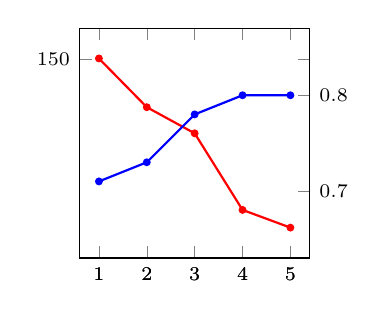
\begin{tikzpicture}

    \begin{axis}[
    width = 4.5cm,
    height= 4.5cm,
    enlarge x limits = 0.1,
    enlarge y limits = 0.1,
    legend columns=3,
    legend style={at={(0.05,-0.3)},anchor=west},
    xmax = 5,
    xtick={1,2,3,4,5},
    xmin = 1,
	ymin= 0,
	ymax=160,
	ytick={150,200},
	%ymode = log,
]
\addplot[thick, red, mark=*,
mark options={scale=0.5},
]
	plot coordinates {
		(1, 150.75)
		(2, 110.03)
		(3, 88.19)
		(4, 24.2)
		(5, 9.4)
	};
%\addlegendentry{search time}
\end{axis}

\begin{axis}[
    width = 4.5cm,
    height= 4.5cm,
	axis y line*=right,
    enlarge x limits = 0.1,
    enlarge y limits = 0.1,
    legend columns=3,
    legend style={at={(0.05,-0.3)},anchor=west},
    xmax = 5,
    xtick={1,2,3,4,5},
    xmin = 1,
	ymin=0.65,
	ymax=0.85,
]
\addplot[thick, blue, mark=*,
mark options={scale=0.5},
]
	plot coordinates {
		(1, 0.71)
		(2, 0.73)
		(3, 0.78)
		(4, 0.8)
		(5, 0.8)
	};
%\addlegendentry{coverage}
\end{axis}


\end{tikzpicture}

}
\end{minipage} &
\begin{minipage}{0.25\textwidth}
\resizebox{!}{3.0cm}{

    \begin{axis}[
    width = 5cm,
    height= 5cm,
    enlarge x limits = 0.1,
    enlarge y limits = 0.1,
    legend columns=3,
    legend style={at={(0.05,-0.3)},anchor=west},
    xmax = 5,
    xtick={1,2,3,4,5},
    xmin = 1,
	title = \#MUGS,
]
\addplot[thick, red, mark=*,
mark options={scale=0.5},
]
	plot coordinates {
		(1, 4.77)
		(2, 3.27)
		(3, 2.38)
		(4, 1.85)
		(5, 1.45)
	};
    \end{axis}

\end{tikzpicture}
\vspace{0.7cm}
\\

}
\end{minipage}
\end{tabular}
\vspace{-0.3cm}
\caption{\label{fig:ipc-local} Local explanation results on IPC 
benchmarks, cost bound $0.75$, for SysW as a function of $|A|$. Left:
coverage, \ie, fraction of solved questions (dashed, right y-axis);
%
%OSP (dotted), \hlmcut (dashed dotted) (right y-axis)
%
and average runtime (solid, left y-axis). Right: average \#MUGS.}
%\joerg{integrate reference point coverage as horizontal lines into the left plot}
%\rebecca{update plot with new benchmark results with all ICP instances}
%
\vspace{-0.55cm}
\end{figure}


%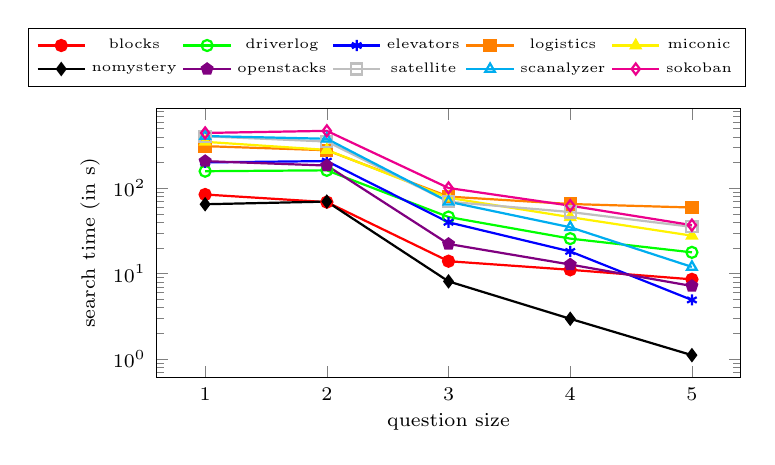
\begin{tikzpicture}[scale=1]
\tiny
    \begin{axis}[
    width = 9cm,
    height=5cm,
    enlarge x limits = 0.1,
    enlarge y limits = 0.1,
    ymode=log,
    xmin = 1,
	xmax = 5,
	xtick={1,2,3,4,5},
	xlabel = {question size},
	x label style = {font=\scriptsize},
	ylabel = {search time (in s)},
	legend style={at={(1.01,1.30)}},
	y label style = {font=\scriptsize},
	legend columns=5,
	x tick label style = {font=\scriptsize, yshift=-0.05cm},
	y tick label style = {font=\scriptsize, xshift=-0.05cm},
]
\addplot[thick, red, mark=*,
]
	plot coordinates {
		(1, 84.53)
		(2, 68.87)
		(3, 13.99)
		(4, 11.1)
		(5, 8.58)
	};
\addlegendentry{blocks}
\addplot[thick, green, mark=o,
]
	plot coordinates {
		(1, 158.49)
		(2, 162.32)
		(3, 46.09)
		(4, 25.74)
		(5, 17.77)
	};
\addlegendentry{driverlog}
\addplot[thick, blue, mark=asterisk,
]
	plot coordinates {
		(1, 201.02)
		(2, 208.31)
		(3, 39.96)
		(4, 18.21)
		(5, 4.92)
	};
\addlegendentry{elevators}
\addplot[thick, orange, mark=square*,
]
	plot coordinates {
		(1, 311.58)
		(2, 279.05)
		(3, 79.89)
		(4, 65.44)
		(5, 59.51)
	};
\addlegendentry{logistics}
\addplot[thick, yellow, mark=triangle*,
]
	plot coordinates {
		(1, 350.17)
		(2, 281.58)
		(3, 77.4)
		(4, 45.93)
		(5, 27.85)
	};
\addlegendentry{miconic}
\addplot[thick, black, mark=diamond*,
]
	plot coordinates {
		(1, 65.03)
		(2, 69.83)
		(3, 8.12)
		(4, 2.96)
		(5, 1.11)
	};
\addlegendentry{nomystery}
\addplot[thick, violet, mark=pentagon*,
]
	plot coordinates {
		(1, 208.06)
		(2, 184.65)
		(3, 22.27)
		(4, 12.79)
		(5, 7.17)
	};
\addlegendentry{openstacks}
\addplot[thick, lightgray, mark=square,
]
	plot coordinates {
		(1, 406.77)
		(2, 352.83)
		(3, 69.58)
		(4, 52.73)
		(5, 35.34)
	};
\addlegendentry{satellite}
\addplot[thick, cyan, mark=triangle,
]
	plot coordinates {
		(1, 409.17)
		(2, 380.07)
		(3, 69.56)
		(4, 34.95)
		(5, 12.0)
	};
\addlegendentry{scanalyzer}
\addplot[thick, magenta, mark=diamond,
]
	plot coordinates {
		(1, 444.74)
		(2, 470.68)
		(3, 100.78)
		(4, 62.61)
		(5, 37.0)
	};
\addlegendentry{sokoban}

    \end{axis}

\end{tikzpicture}
\\

%
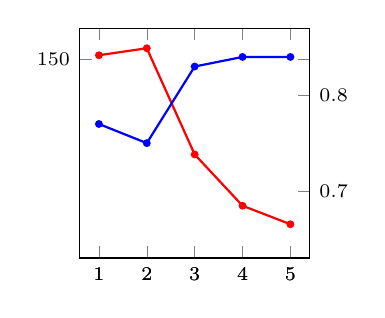
\begin{tikzpicture}

    \begin{axis}[
    width = 4.5cm,
    height= 4.5cm,
    enlarge x limits = 0.1,
    enlarge y limits = 0.1,
    legend columns=3,
    legend style={at={(0.05,-0.2)},anchor=west},
    xmin = 1,
    xmax = 5,
    xtick={1,2,3,4,5},
	ymin= 120,
	ymax=220,
	ymin= 0,
	ymax=160,
	ytick={150,200},
	%ymode = log,
]
	\addplot[thick, red, mark=*, mark options={scale=0.5}]
		plot coordinates {
			(1, 153.43)
			(2, 159.28)
			(3, 70.55)
			(4, 27.7)
			(5, 12.22)
		};
%\addlegendentry{search time}

\end{axis}

\begin{axis}[
    width = 4.5cm,
    height= 4.5cm,
	axis y line*=right,
    enlarge x limits = 0.1,
    enlarge y limits = 0.1,
    legend columns=3,
    legend style={at={(0.5,-0.2)},anchor=west},
    xmax = 5,
    xtick={1,2,3,4,5},
    xmin = 1,
	ymin=0.65,
	ymax=0.85,
]
	\addplot[thick, blue, mark=*, mark options={scale=0.5}]
		plot coordinates {
			(1, 0.77)
			(2, 0.75)
			(3, 0.83)
			(4, 0.84)
			(5, 0.84)
		};
%\addlegendentry{coverage}
\end{axis}

\end{tikzpicture}


These results are consistent across domains, and are much stronger in
some cases.
%
For example, while for $|A|=1$ our coverage is higher than that
of \hlmcut\ in only 2 domains here, for $|A|=5$ that is so in 6
domains. Compared against OSP, the number of domains with higher
coverage rises from 5 to 13.
%
% Joerg: previous snippets
%
%% %% Of the 42 domains that have at least one instance with $\geq 6$
%% %% goals,
%% %
%% In particular, six domains have $> 20\%$ increases in coverage from
%% $|A|=1$ to $|A|=5$.
%% %
%% % Joerg: no need for this, runtime even on average here decreases by
%% % orders of magnitude.
%% %
%% %% and in 15 domains average runtime decreases by at least one order
%% %% of magnitude.
%% %
%% For $|A|=5$, coverage is $\geq$ that of \hlmcut\ in 6 domains and
%% $\geq$ that of OSP in 12 domains.\joerg{are these numbers correct?
%% even in the table I count like 10 domains where we surpass lmcut for
%% 0.75. also, we should compare these numbers to those for global
%% explanation ie the table}
%
The average number of MUGS for $|A|=5$ is $<6$ in all domains except
\parcprinter\ ($6.29$), \openstacks\ ($9.35$), \woodworking\ ($13.43$), 
and \visitall\ ($20.16$).
%
%% The average number of MUGS for $|A|=5$ is $<5$ in all domains,
%% including ones like Floortile, Gripper, Miconic, Woodworking, where
%% global explanations can be large as shown in
%% Figure~\ref{table:coverage_ipc}.

%% For coverage, Blocksworld, Depots, Elevators, NoMystery, Openstacks, Visiteal
%
%% runtime: 
%%1 order blocks, drive, floortile, elevators, grip,
%% mic, log, nomystrey, pathway, sat, soko, stor, tetr, tpp,
%% transp, wood; 
%% 2 orders depots, scan, trucks




%%%%%%%%%%%%%%%%%%%%%%%%%%%%%%%%%%%%%%%%%%%%%%%%%%%%%%%%%%%%%%%%%%%%
%%%%%%%%%%%%%%%%%%%%%%%%%%%%%%%%%%%%%%%%%%%%%%%%%%%%%%%%%%%%%%%%%%%%
%%%%%%%%%%%%%%%%%%%%%%%%%%%%%%%%%%%%%%%%%%%%%%%%%%%%%%%%%%%%%%%%%%%%
%%%% Action-Set Properties

\subsection{Action-Set Properties}
\label{experiments:asp}

%% \joerg{notes reg data: SysS better for 1.0, SysW better elsewhere. 
%% fig 3 show 1.5 (compared to 1.25 blocks looks way better, nomyst looks
%% way better, rovers presumably similar, tpp only marginally worse; in
%% 1.0, there's not much to see and it's not good to show a case at the
%% extreme end of the sopectrum). in fig 4, show 1.25 or 1.5 (in 1.0,
%% would have to use SysS not SysW, coverage there is boring); probably
%% add sentence in text reg flat MUGS curves for TPP (and nomystery 1.5)
%% due to large solvable property sets, and for Rovers due to small
%% unsolvable property sets.}
%% %
%% \joerg{actually, decided to show 1.0 instead, based on the reason that, 
%% there, the benchmarks are most interesting as far as MUGS analysis is
%% concerned: for higher C values, in NoMystery and TPP very large
%% property subsets are solvable.}
%% %
%% \joerg{in TR, we can incude the exact same figures, just all of them 
%% not only 1}

To evaluate the use of our framework with more complex plan
properties, we experimented with the compilation of action-set
properties as per Section~\ref{actionsetprops}.
%
We extended four domains with action-set properties: NoMystery,
Rovers, and TPP as per \cite{nakhost:etal:icaps-12}, with controlled
resource constrainedness (\cf\ Section~\ref{background}); plus the
Blocksworld as an intuitively differently structured domain.
%
In NoMystery, the action-set properties are as in our illustrative
example. In Rovers, the properties ask which rover or camera is used
for which observation. In TPP, they ask which road segments are used,
and which goods are bought at which markets. In Blocksworld, we
include two hands and the properties ask which hand is used for which
blocks.
%
We set the original goal facts as hard goals, so that the analysis
determines exclusion relations over conjunctions of action-set
properties.

We encoded resource consumption into the FDR state variables, enabling
the use of trap learning which turns out to be highly beneficial
here. We generated benchmarks of sizes around the feasibility
borderline, and we experimented with resource constrainedness
$x \in \{1.0, 1.25, 1.5, 2.0\}$. For reference, we ran \astar\
with \hlmcut\ as before, on all goal facts (original plus compiled
action-set properties). Current OSP planners cannot handle hard goals,
so we used our base planner with trap learning instead as a second
reference point.

%% \joerg{presumably, include a figure with one plot per domain,
%% fixing number of goals as in IJCAI long versions (main paper plot),
%% and with fixed constrainedness factor x. use same x for both global
%% and local explanations. x=2.0 is too high, Blocks and TPP
%% apparently typically all goals achievable easil for base
%% planner. x=1.0 shows off advantage of trap learning, but does not
%% challenge the reference points enough. for x=1.5 on the other hand
%% trap learning is way less important than for 1.0. Try x=1.25 and
%% see what it looks like.}
%
\begin{figure}[h!]
\vspace{-0.3cm}
\small
\centering

\tiny
\centering
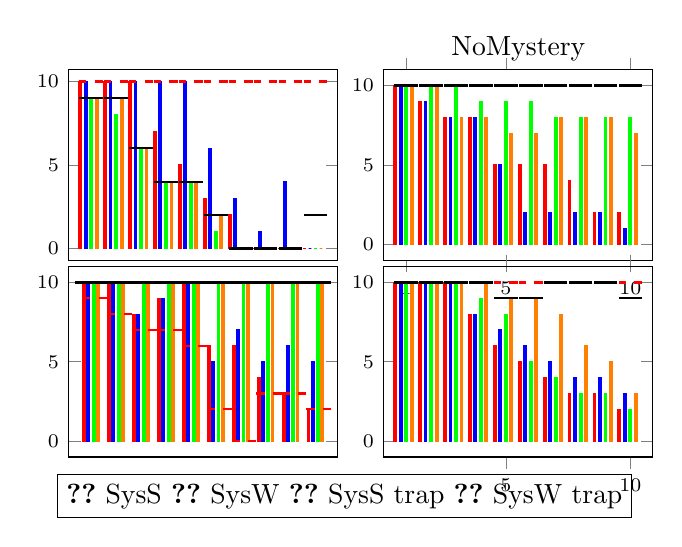
\begin{tikzpicture}
    \begin{axis}[
    width = 5cm,
    height=4cm,
    enlarge x limits = 0.1,
    enlarge y limits = 0.07,
    legend columns=1,
    ybar,
    bar width=1pt,
    ymin = 0,
    ymax = 10,
	compat=1.6,
	title={},
	xticklabels={,,},
	xtick style={draw=none},
	%ylabel=goals 06,
	at={(0,0)},
]
\addplot+[ybar, bar shift =-4.0pt, red,
]
plot coordinates {
(07, 2) %c_125
(08, 0) %c_125
(03, 10) %c_125
(10, 0) %c_125
(06, 3) %c_125
(09, 0) %c_125
(02, 10) %c_125
(05, 5) %c_125
(04, 7) %c_125
(01, 10) %c_125
};
\label{plot:props_hff_bu_53}
\addplot+[ybar, bar shift =-2.0pt, blue,
]
plot coordinates {
(07, 3) %c_125
(08, 1) %c_125
(03, 10) %c_125
(10, 0) %c_125
(06, 6) %c_125
(09, 4) %c_125
(02, 10) %c_125
(05, 10) %c_125
(04, 10) %c_125
(01, 10) %c_125
};
\label{plot:props_hff_td_53}
\addplot+[ybar, bar shift =0.0pt, green,
]
plot coordinates {
(07, 0) %c_125
(08, 0) %c_125
(03, 6) %c_125
(10, 0) %c_125
(06, 1) %c_125
(09, 0) %c_125
(02, 8) %c_125
(05, 4) %c_125
(04, 4) %c_125
(01, 9) %c_125
};
\label{plot:props_trap_bu_53}
\addplot+[ybar, bar shift =2.0pt, orange,
]
plot coordinates {
(07, 0) %c_125
(08, 0) %c_125
(03, 6) %c_125
(10, 0) %c_125
(06, 2) %c_125
(09, 0) %c_125
(02, 9) %c_125
(05, 4) %c_125
(04, 4) %c_125
(01, 9) %c_125
};
\label{plot:props_trap_td_53}

%lmcut
\addplot+[only marks, mark = -, mark options = {thick, red, dashed}, mark size = 0.15cm, black,
]
plot coordinates {
(02, 10)
(01, 10)
(04, 10)
(03, 10)
(07, 10)
(08, 10)
(06, 10)
(10, 10)
(05, 10)
(09, 10)
};

%trap first meta node top down
\addplot+[only marks, mark = -, mark options = {thick, black}, mark size = 0.15cm, black,
]
plot coordinates {
(01, 9)
(02, 9)
(03, 6)
(04, 4)
(05, 4)
(06, 2)
(07, 0)
(08, 0)
(09, 0)
(10, 2)
};
    \end{axis}
    \hfill
    
%\node[draw, align=center] (test) at (2,-2) {
%\ref{plot:props_hff_bu_53} props-hff-bu\\
%\ref{plot:props_hff_td_53} props-hff-td\\
%\ref{plot:props_trap_bu_53} props-trap-bu\\
%\ref{plot:props_trap_td_53} props-trap-td\\
%};




    \begin{axis}[
    width = 5cm,
    height=4cm,
    enlarge x limits = 0.1,
    enlarge y limits = 0.1,
    legend columns=1,
    ybar,
    bar width=1pt,
    ymin = 0,
    ymax = 10,
	compat=1.6,
	title=NoMystery,
	title style={yshift=-1.5ex},
	%ylabel=goals 6,
	%xticklabels={,,},
	%xtick style={draw=none},
	xtick= {1,5,10},
	at={(4cm,0)},
]
\addplot+[ybar, bar shift =-4.0pt, red,
]
plot coordinates {
(04, 8) %c_100
(09, 2) %c_100
(10, 2) %c_100
(08, 4) %c_100
(02, 9) %c_100
(07, 5) %c_100
(06, 5) %c_100
(05, 5) %c_100
(03, 8) %c_100
(01, 10) %c_100
};
\label{plot:props_bu_hff_46}
\addplot+[ybar, bar shift =-2.0pt, blue,
]
plot coordinates {
(04, 8) %c_100
(09, 2) %c_100
(10, 1) %c_100
(08, 2) %c_100
(02, 9) %c_100
(07, 2) %c_100
(06, 2) %c_100
(05, 5) %c_100
(03, 8) %c_100
(01, 10) %c_100
};
\label{plot:props_td_hff_46}
\addplot+[ybar, bar shift =0.0pt, green,
]
plot coordinates {
(04, 9) %c_100
(09, 8) %c_100
(10, 8) %c_100
(08, 8) %c_100
(02, 10) %c_100
(07, 8) %c_100
(06, 9) %c_100
(05, 9) %c_100
(03, 10) %c_100
(01, 10) %c_100
};
\label{plot:props_bu_trap_46}
\addplot+[ybar, bar shift =2.0pt, orange,
]
plot coordinates {
(04, 8) %c_100
(09, 8) %c_100
(03, 8) %c_100
(08, 8) %c_100
(02, 10) %c_100
(07, 8) %c_100
(06, 7) %c_100
(05, 7) %c_100
(10, 7) %c_100
(01, 10) %c_100
};
\label{plot:props_td_trap_46}

%lmcut
\addplot+[only marks, mark = -, mark options = {thick, red, dashed}, mark size = 0.15cm, black,
]
plot coordinates {
(01, 10)
(02, 10)
(03, 10)
(04, 10)
(05, 10)
(06, 10)
(07, 10)
(08, 10)
(09, 10)
(10, 10)
};

%trap first meta node top down
\addplot+[only marks, mark = -, mark options = {thick, black}, mark size = 0.15cm, black,
]
plot coordinates {
(01, 10)
(02, 10)
(03, 10)
(04, 10)
(05, 10)
(06, 10)
(07, 10)
(08, 10)
(09, 10)
(10, 10)
};
    \end{axis}
    \hfill
    
%\node[draw, align=center] (test) at (8,-18) {
%\ref{plot:props_bu_hff_46} props-bu-hff\\
%\ref{plot:props_td_hff_46} props-td-hff\\
%\ref{plot:props_bu_trap_46} props-bu-trap\\
%\ref{plot:props_td_trap_46} props-td-trap\\
%};




\begin{axis}[
width = 5cm,
height=4cm,
enlarge x limits = 0.1,
enlarge y limits = 0.1,
legend columns=1,
ybar,
bar width=1pt,
ymin = 0,
ymax = 10,
compat=1.6,
at={(0,-2.5cm)},
	xticklabels={,,},
	xtick style={draw=none},
]
\addplot+[ybar, bar shift =-2.5pt, red,
]
plot coordinates {
(08, 4)
(09, 3)
(01, 10)
(03, 8)
(02, 10)
(04, 9)
(05, 10)
(06, 6)
(10, 2)
(07, 6)
};
\label{plot:properties_hff_bu_52}
\addplot+[ybar, bar shift =-1.0pt, blue,
]
plot coordinates {
(01, 10)
(08, 5)
(02, 10)
(04, 9)
(03, 8)
(05, 10)
(06, 5)
(10, 5)
(07, 7)
(09, 6)
};
\label{plot:properties_hff_td_52}
\addplot+[ybar, bar shift =1.0pt, green,
]
plot coordinates {
(09, 10)
(01, 10)
(02, 10)
(04, 10)
(03, 10)
(05, 10)
(06, 10)
(10, 10)
(07, 10)
(08, 10)
};
\label{plot:properties_trap_prefop_bu_52}
\addplot+[ybar, bar shift =2.5pt, orange,
]
plot coordinates {
(01, 10)
(08, 10)
(02, 10)
(03, 10)
(04, 10)
(05, 10)
(06, 10)
(10, 10)
(07, 10)
(09, 10)
};
\label{plot:properties_trap_prefop_td_52}

%start node sysW
\addplot+[only marks, mark = -, mark options = {thick}, mark size = 0.2cm, black,
]
plot coordinates {
(02, 10)
(01, 10)
(04, 10)
(03, 10)
(07, 10)
(08, 10)
(06, 10)
(10, 10)
(05, 10)
(09, 10)
};
%optimal
\addplot+[only marks, mark = -, mark options = {thick, red, dashed}, mark size = 0.2cm, black,
]
plot coordinates {
(03, 7)
(05, 6)
(07, 0)
(09, 3)
(01, 9)
(02, 8)
(04, 7)
(06, 2)
(08, 3)
(10, 2)
};

\end{axis}



    \begin{axis}[
    width = 5cm,
    height=4cm,
    enlarge x limits = 0.1,
    enlarge y limits = 0.1,
    legend columns=1,
    ybar,
    bar width=1pt,
    ymin = 0,
    ymax = 10,
compat=1.6,
%title=c 150,
%ylabel=goals 7,
at={(4cm,-2.5cm)},
]
\addplot+[ybar, bar shift =-4.0pt, red,
]
plot coordinates {
(07, 4) %c_150
(06, 5) %c_150
(05, 6) %c_150
(09, 3) %c_150
(08, 3) %c_150
(10, 2) %c_150
(01, 10) %c_150
(04, 8) %c_150
(03, 10) %c_150
(02, 10) %c_150
};
\label{plot:props_bu_hff_49}
\addplot+[ybar, bar shift =-2.0pt, blue,
]
plot coordinates {
(07, 5) %c_150
(06, 6) %c_150
(05, 7) %c_150
(09, 4) %c_150
(08, 4) %c_150
(10, 3) %c_150
(01, 10) %c_150
(04, 8) %c_150
(03, 10) %c_150
(02, 10) %c_150
};
\label{plot:props_td_hff_49}
\addplot+[ybar, bar shift =0.0pt, green,
]
plot coordinates {
(07, 4) %c_150
(06, 5) %c_150
(05, 8) %c_150
(09, 3) %c_150
(08, 3) %c_150
(03, 10) %c_150
(01, 10) %c_150
(04, 9) %c_150
(10, 2) %c_150
(02, 10) %c_150
};
\label{plot:props_bu_trap_49}
\addplot+[ybar, bar shift =2.0pt, orange,
]
plot coordinates {
(07, 8) %c_150
(06, 9) %c_150
(05, 9) %c_150
(09, 5) %c_150
(08, 6) %c_150
(10, 3) %c_150
(01, 10) %c_150
(04, 10) %c_150
(03, 10) %c_150
(02, 10) %c_150
};
\label{plot:props_td_trap_49}

%lmcut
\addplot+[only marks, mark = -, mark options = {thick, red, dashed}, mark size = 0.15cm, black,
]
plot coordinates {
(02, 10)
(01, 10)
(04, 10)
(03, 10)
(07, 10)
(08, 10)
(06, 10)
(10, 10)
(05, 10)
(09, 10)
};

%trap first meta node top down
\addplot+[only marks, mark = -, mark options = {thick, black}, mark size = 0.15cm, black,
]
plot coordinates {
(01, 10)
(02, 10)
(03, 10)
(04, 10)
(05, 9)
(06, 9)
(07, 10)
(08, 10)
(09, 10)
(10, 9)
};
    \end{axis}
    \hfill
    
%\node[draw, align=center] (test) at (8,-18) {
%\ref{plot:props_bu_hff_49} props-bu-hff\\
%\ref{plot:props_td_hff_49} props-td-hff\\
%\ref{plot:props_bu_trap_49} props-bu-trap\\
%\ref{plot:props_td_trap_49} props-td-trap\\
%};




\node[draw] (test) at (3.5,-3.0) {
\ref{plot:props_bu_hff_94}   SysS
\ref{plot:props_td_hff_94}   SysW
\ref{plot:props_bu_trap_94} SysS trap 
\ref{plot:props_td_trap_94} SysW trap 
%\ref{plot:baseline_lmcut} \hlmcut
%\ref{plot:baseline_sysW_node} trap
};
\end{tikzpicture}

\vspace{-0.25cm}
\caption{\label{fig:asp-global} Coverage for global action-set 
property explanation at $x=1.0$.  Number of properties on x-axis,
scaling from $1$ to $10$. SysS with trap learning. Blocksworld top
left, NoMystery top right, Rovers bottom left, TPP bottom
right.
%\joerg{include reference point data everywhere; include reference points in plot legend}
}
%
% Joerg: easier to include ref points everywhere
%
%% Reference point coverage is 10 and hence not shown, except
%% for \hlmcut\ in Rovers (red dashed line near bottom).
%
\vspace{-0.3cm}
\end{figure}

For lack of space, we show only the data for $x = 1.0$, where our
benchmarks are most interesting in that, for higher amounts of
available resources, in NoMystery and TPP almost all property subsets
are solvable.
%
Figure~\ref{fig:asp-global} shows that computing global action-set
property explanations is feasible, at $x=1.0$, compared to the
reference points. SysS with trap learning matches reference point
coverage except for moderate losses in NoMystery.
%
Figure~\ref{fig:asp-local} shows that, as before, the analysis becomes
much easier for local explanation as a function of question size.
%
Rovers is a special case as, there, all pairs of action-set properties
are unsolvable.
%
Given more resources, $x \in \{1.25, 1.5, 2.0\}$, 
%
% Joerg: not as relevant, focus on trap learning
%
% SysW outperforms SysS, 
%
similarly to Figure~\ref{table:coverage_ipc} MUGS analysis becomes
much harder, and the coverage gap to the reference points increases
except in Rovers.\ifdefined\suppflagdefined\else\footnote{We intend to
buy additional pages to include the data for $x > 1$. For AAAI'20
review, the data is in supplementary material at
{\scriptsize \url{https://www.dropbox.com/sh/boq29booqajj7ab/AACbKpiR6jdbeEzCldrvLfk4a?dl=0}}}\fi\
%
\ifdefined\suppflagdefined
%
The data is included in Appendix~\ref{apendix:data}.
%
\fi


\begin{figure}[t]
\vspace{-0.0cm}
\small
\centering

%Search time
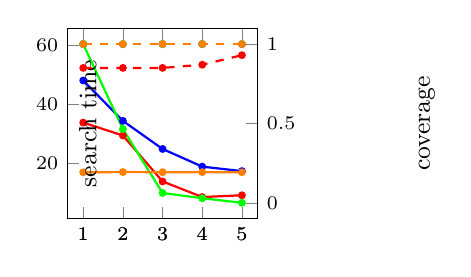
\begin{tikzpicture}
\small
    \begin{axis}[
    width = 4cm,
    height= 4cm,
    enlarge x limits = 0.1,
    enlarge y limits = 0.1,
    legend columns=3,
    legend style={at={(0.05,-0.3)},anchor=west},
    xmax = 5,
    xtick={1,2,3,4,5},
    xmin = 1,
	ylabel= search time,
	y label style={at={(0.2,0.5)}},
	axis y line*=left,
]

%blocksworld search time
\addplot[thick, blue, mark=*,
mark options={scale=0.5, solid},
]
        plot coordinates {
			(1, 48.04)
			(2, 34.37)
			(3, 24.89)
			(4, 18.92)
			(5, 17.4)
        };

%nomystery search time
\addplot[thick, red, mark=*,
mark options={scale=0.5, solid},
]
        plot coordinates {
			(1, 33.8)
			(2, 29.44)
			(3, 13.91)
			(4, 8.64)
			(5, 9.24)
        };

%tpp search time
\addplot[thick, green, mark=*, mark options={scale=0.5, solid},
]
        plot coordinates {
			(1, 60.33)
			(2, 31.62)
			(3, 10.03)
			(4, 8.24)
			(5, 6.7)
        };


%rovers search time
\addplot[thick, orange, mark=*, mark options={scale=0.5, solid},
]
        plot coordinates {
			(1, 17.0)
			(2, 17.08)
			(3, 17.04)
			(4, 17.06)
			(5, 17.02)
        };
\end{axis}

\begin{axis}[
    width = 4cm,
    height= 4cm,
    enlarge x limits = 0.1,
    enlarge y limits = 0.1,
    legend columns=3,
    legend style={at={(0.05,-0.3)},anchor=west},
    xmax = 5,
    xtick={1,2,3,4,5},
    xmin = 1,
	axis y line*=right,
	ylabel= coverage,
	y label style={at={(1.8,0.5)}},
	ymax = 1,
	ymin = 0,
]

%coverage blocksworld
\addplot[thick, blue, dashed, mark=*,
mark options={scale=0.5, solid},
]
        plot coordinates {
			(1, 1.0)
			(2, 1.0)
			(3, 1.0)
			(4, 1.0)
			(5, 1.0)
        };

%coverage nomystery
\addplot[thick, red, dashed, mark=*,
mark options={scale=0.5, solid},
]
        plot coordinates {
			(1, 0.85)
			(2, 0.85)
			(3, 0.85)
			(4, 0.87)
			(5, 0.93)
        };

%tpp coverage
\addplot[thick, green, dashed, mark=*, mark options={scale=0.5, solid},
]
        plot coordinates {
			(1, 1.0)
			(2, 1.0)
			(3, 1.0)
			(4, 1.0)
			(5, 1.0)
        };

%rovers coverage
\addplot[thick, orange, dashed, mark=*, mark options={scale=0.5, solid},
]
        plot coordinates {
			(1, 1.0)
			(2, 1.0)
			(3, 1.0)
			(4, 1.0)
			(5, 1.0)
        };

    \end{axis}


\end{tikzpicture}
%MUGS
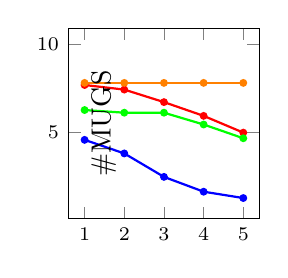
\begin{tikzpicture}

    \begin{axis}[
	%title = \#MUGS,
    width = 4cm,
    height= 4cm,
    enlarge x limits = 0.1,
    enlarge y limits = 0.1,
    legend columns=3,
    legend style={at={(0.05,-0.3)},anchor=west},
    xmax = 5,
    xtick={1,2,3,4,5},
    xmin = 1,
	ymin=1,
	ymax=10,
	ylabel= \#MUGS,
	y label style={at={(0.3,0.5)}},
]

%MUGS blocksworld
\addplot[thick, blue, mark=*,
mark options={scale=0.5, solid},
]
        plot coordinates {
			(1, 4.57)
			(2, 3.8)
			(3, 2.47)
			(4, 1.63)
			(5, 1.27)
        };

%MUGS nomystery
\addplot[thick, red, mark=*,
mark options={scale=0.5, solid},
]
        plot coordinates {
			(1, 7.68)
			(2, 7.42)
			(3, 6.71)
			(4, 5.93)
			(5, 4.98)
        };


%MUGS TPP
\addplot[thick, green, mark=*, mark options={scale=0.5, solid},
]
        plot coordinates {
			(1, 6.26)
			(2, 6.11)
			(3, 6.11)
			(4, 5.44)
			(5, 4.66)
        };

%MUGS rovers
\addplot[thick, orange, mark=*, mark options={scale=0.5, solid},
]
        plot coordinates {
			(1, 7.8)
			(2, 7.8)
			(3, 7.8)
			(4, 7.8)
			(5, 7.8)
        };

\end{axis}
\end{tikzpicture}



\vspace{-0.3cm}
\caption{\label{fig:asp-local} Local action-set property explanation 
at $x=1.0$. SysS with trap learning. Average runtime (left) and
average \#MUGS (right) as a function of $|A|$. Blocksworld solid,
NoMystery dashed, Rovers dotted, TPP dashdotted.
%\joerg{remove coverage}\joerg{replace by b/w readable version?}
}
\vspace{-0.6cm}
\end{figure}



%%%% Action-Set Properties, END SUBMISSION VERSION
%%%%%%%%%%%%%%%%%%%%%%%%%%%%%%%%%%%%%%%%%%%%%%%%%%%%%%%%%%%%%%%%%%%%
%%%%%%%%%%%%%%%%%%%%%%%%%%%%%%%%%%%%%%%%%%%%%%%%%%%%%%%%%%%%%%%%%%%%
%%%%%%%%%%%%%%%%%%%%%%%%%%%%%%%%%%%%%%%%%%%%%%%%%%%%%%%%%%%%%%%%%%%%







%%%%%%%%%%%%%%%%%%%%%%%%%%%%%%%%%%%%%%%%%%%%%%%%%%%%%%%%%%%%%%%%%%%%
%%%%%%%%%%%%%%%%%%%%%%%%%%%%%%%%%%%%%%%%%%%%%%%%%%%%%%%%%%%%%%%%%%%%
%%%%%%%%%%%%%%%%%%%%%%%%%%%%%%%%%%%%%%%%%%%%%%%%%%%%%%%%%%%%%%%%%%%%
%%%% IJCAI SUPPLEMENTARY MATERIAL VERSION

%% \ifdefined\suppflagdefined

%% \subsection{Action-Set Properties}

%% \begin{figure*}[htb]
%% \centering\centering
%% %\newlength{\mywidth}
\setlength{\mywidth}{16.5cm}

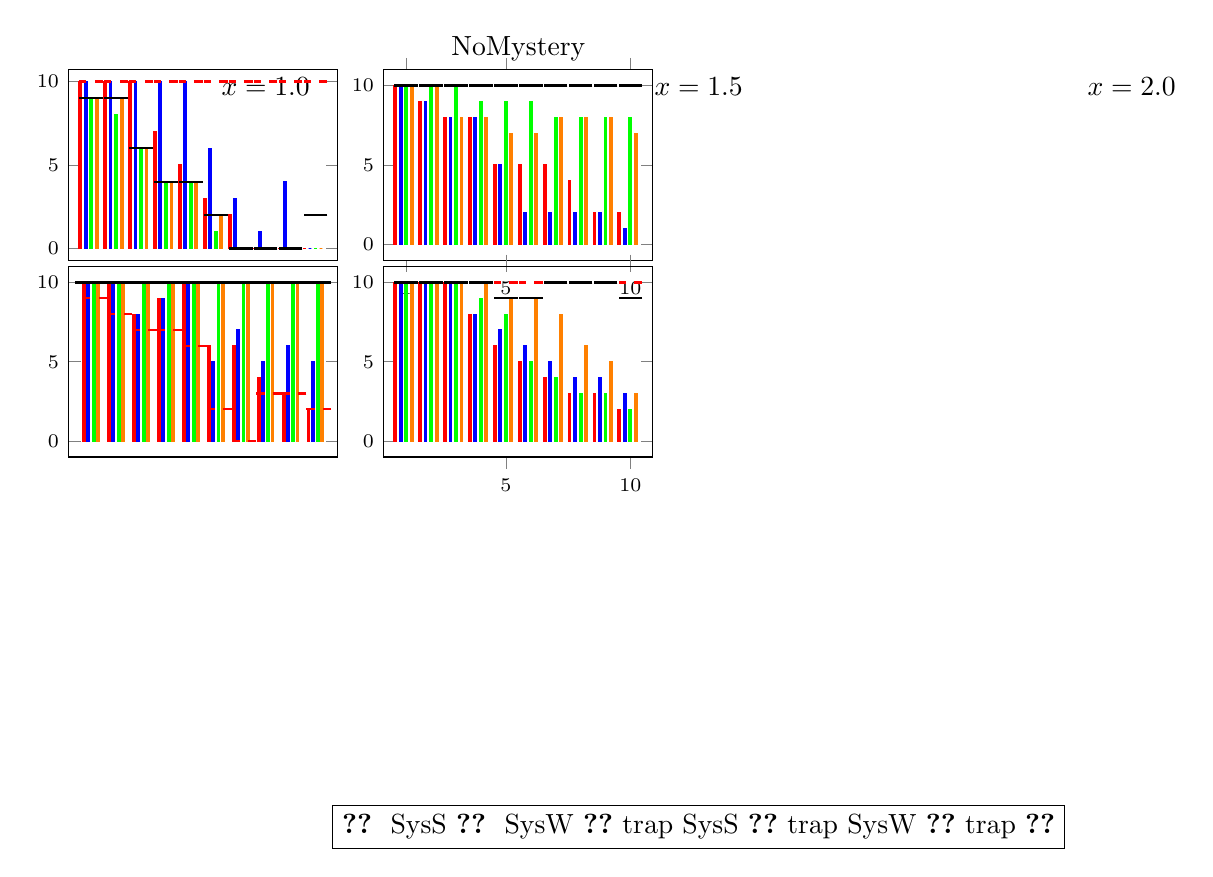
\begin{tikzpicture}
\node[] (c1) at (2.5,2.2) {$x=1.0$};
\node[] (c15) at (8,2.2) {$x=1.5$};
\node[] (c2) at (13.5,2.2) {$x=2.0$};


    \begin{axis}[
    width = 5cm,
    height=4cm,
    enlarge x limits = 0.1,
    enlarge y limits = 0.07,
    legend columns=1,
    ybar,
    bar width=1pt,
    ymin = 0,
    ymax = 10,
	compat=1.6,
	title={},
	xticklabels={,,},
	xtick style={draw=none},
	%ylabel=goals 06,
	at={(0,0)},
]
\addplot+[ybar, bar shift =-4.0pt, red,
]
plot coordinates {
(07, 2) %c_125
(08, 0) %c_125
(03, 10) %c_125
(10, 0) %c_125
(06, 3) %c_125
(09, 0) %c_125
(02, 10) %c_125
(05, 5) %c_125
(04, 7) %c_125
(01, 10) %c_125
};
\label{plot:props_hff_bu_53}
\addplot+[ybar, bar shift =-2.0pt, blue,
]
plot coordinates {
(07, 3) %c_125
(08, 1) %c_125
(03, 10) %c_125
(10, 0) %c_125
(06, 6) %c_125
(09, 4) %c_125
(02, 10) %c_125
(05, 10) %c_125
(04, 10) %c_125
(01, 10) %c_125
};
\label{plot:props_hff_td_53}
\addplot+[ybar, bar shift =0.0pt, green,
]
plot coordinates {
(07, 0) %c_125
(08, 0) %c_125
(03, 6) %c_125
(10, 0) %c_125
(06, 1) %c_125
(09, 0) %c_125
(02, 8) %c_125
(05, 4) %c_125
(04, 4) %c_125
(01, 9) %c_125
};
\label{plot:props_trap_bu_53}
\addplot+[ybar, bar shift =2.0pt, orange,
]
plot coordinates {
(07, 0) %c_125
(08, 0) %c_125
(03, 6) %c_125
(10, 0) %c_125
(06, 2) %c_125
(09, 0) %c_125
(02, 9) %c_125
(05, 4) %c_125
(04, 4) %c_125
(01, 9) %c_125
};
\label{plot:props_trap_td_53}

%lmcut
\addplot+[only marks, mark = -, mark options = {thick, red, dashed}, mark size = 0.15cm, black,
]
plot coordinates {
(02, 10)
(01, 10)
(04, 10)
(03, 10)
(07, 10)
(08, 10)
(06, 10)
(10, 10)
(05, 10)
(09, 10)
};

%trap first meta node top down
\addplot+[only marks, mark = -, mark options = {thick, black}, mark size = 0.15cm, black,
]
plot coordinates {
(01, 9)
(02, 9)
(03, 6)
(04, 4)
(05, 4)
(06, 2)
(07, 0)
(08, 0)
(09, 0)
(10, 2)
};
    \end{axis}
    \hfill
    
%\node[draw, align=center] (test) at (2,-2) {
%\ref{plot:props_hff_bu_53} props-hff-bu\\
%\ref{plot:props_hff_td_53} props-hff-td\\
%\ref{plot:props_trap_bu_53} props-trap-bu\\
%\ref{plot:props_trap_td_53} props-trap-td\\
%};



    \begin{axis}[
    width = 5cm,
    height=4cm,
    enlarge x limits = 0.1,
    enlarge y limits = 0.1,
    legend columns=1,
    ybar,
    bar width=1pt,
    ymin = 0,
    ymax = 10,
	compat=1.6,
	title=NoMystery,
	title style={yshift=-1.5ex},
	%ylabel=goals 6,
	%xticklabels={,,},
	%xtick style={draw=none},
	xtick= {1,5,10},
	at={(4cm,0)},
]
\addplot+[ybar, bar shift =-4.0pt, red,
]
plot coordinates {
(04, 8) %c_100
(09, 2) %c_100
(10, 2) %c_100
(08, 4) %c_100
(02, 9) %c_100
(07, 5) %c_100
(06, 5) %c_100
(05, 5) %c_100
(03, 8) %c_100
(01, 10) %c_100
};
\label{plot:props_bu_hff_46}
\addplot+[ybar, bar shift =-2.0pt, blue,
]
plot coordinates {
(04, 8) %c_100
(09, 2) %c_100
(10, 1) %c_100
(08, 2) %c_100
(02, 9) %c_100
(07, 2) %c_100
(06, 2) %c_100
(05, 5) %c_100
(03, 8) %c_100
(01, 10) %c_100
};
\label{plot:props_td_hff_46}
\addplot+[ybar, bar shift =0.0pt, green,
]
plot coordinates {
(04, 9) %c_100
(09, 8) %c_100
(10, 8) %c_100
(08, 8) %c_100
(02, 10) %c_100
(07, 8) %c_100
(06, 9) %c_100
(05, 9) %c_100
(03, 10) %c_100
(01, 10) %c_100
};
\label{plot:props_bu_trap_46}
\addplot+[ybar, bar shift =2.0pt, orange,
]
plot coordinates {
(04, 8) %c_100
(09, 8) %c_100
(03, 8) %c_100
(08, 8) %c_100
(02, 10) %c_100
(07, 8) %c_100
(06, 7) %c_100
(05, 7) %c_100
(10, 7) %c_100
(01, 10) %c_100
};
\label{plot:props_td_trap_46}

%lmcut
\addplot+[only marks, mark = -, mark options = {thick, red, dashed}, mark size = 0.15cm, black,
]
plot coordinates {
(01, 10)
(02, 10)
(03, 10)
(04, 10)
(05, 10)
(06, 10)
(07, 10)
(08, 10)
(09, 10)
(10, 10)
};

%trap first meta node top down
\addplot+[only marks, mark = -, mark options = {thick, black}, mark size = 0.15cm, black,
]
plot coordinates {
(01, 10)
(02, 10)
(03, 10)
(04, 10)
(05, 10)
(06, 10)
(07, 10)
(08, 10)
(09, 10)
(10, 10)
};
    \end{axis}
    \hfill
    
%\node[draw, align=center] (test) at (8,-18) {
%\ref{plot:props_bu_hff_46} props-bu-hff\\
%\ref{plot:props_td_hff_46} props-td-hff\\
%\ref{plot:props_bu_trap_46} props-bu-trap\\
%\ref{plot:props_td_trap_46} props-td-trap\\
%};



\begin{axis}[
width = 5cm,
height=4cm,
enlarge x limits = 0.1,
enlarge y limits = 0.1,
legend columns=1,
ybar,
bar width=1pt,
ymin = 0,
ymax = 10,
compat=1.6,
at={(0,-2.5cm)},
	xticklabels={,,},
	xtick style={draw=none},
]
\addplot+[ybar, bar shift =-2.5pt, red,
]
plot coordinates {
(08, 4)
(09, 3)
(01, 10)
(03, 8)
(02, 10)
(04, 9)
(05, 10)
(06, 6)
(10, 2)
(07, 6)
};
\label{plot:properties_hff_bu_52}
\addplot+[ybar, bar shift =-1.0pt, blue,
]
plot coordinates {
(01, 10)
(08, 5)
(02, 10)
(04, 9)
(03, 8)
(05, 10)
(06, 5)
(10, 5)
(07, 7)
(09, 6)
};
\label{plot:properties_hff_td_52}
\addplot+[ybar, bar shift =1.0pt, green,
]
plot coordinates {
(09, 10)
(01, 10)
(02, 10)
(04, 10)
(03, 10)
(05, 10)
(06, 10)
(10, 10)
(07, 10)
(08, 10)
};
\label{plot:properties_trap_prefop_bu_52}
\addplot+[ybar, bar shift =2.5pt, orange,
]
plot coordinates {
(01, 10)
(08, 10)
(02, 10)
(03, 10)
(04, 10)
(05, 10)
(06, 10)
(10, 10)
(07, 10)
(09, 10)
};
\label{plot:properties_trap_prefop_td_52}

%start node sysW
\addplot+[only marks, mark = -, mark options = {thick}, mark size = 0.2cm, black,
]
plot coordinates {
(02, 10)
(01, 10)
(04, 10)
(03, 10)
(07, 10)
(08, 10)
(06, 10)
(10, 10)
(05, 10)
(09, 10)
};
%optimal
\addplot+[only marks, mark = -, mark options = {thick, red, dashed}, mark size = 0.2cm, black,
]
plot coordinates {
(03, 7)
(05, 6)
(07, 0)
(09, 3)
(01, 9)
(02, 8)
(04, 7)
(06, 2)
(08, 3)
(10, 2)
};

\end{axis}


    \begin{axis}[
    width = 5cm,
    height=4cm,
    enlarge x limits = 0.1,
    enlarge y limits = 0.1,
    legend columns=1,
    ybar,
    bar width=1pt,
    ymin = 0,
    ymax = 10,
compat=1.6,
%title=c 150,
%ylabel=goals 7,
at={(4cm,-2.5cm)},
]
\addplot+[ybar, bar shift =-4.0pt, red,
]
plot coordinates {
(07, 4) %c_150
(06, 5) %c_150
(05, 6) %c_150
(09, 3) %c_150
(08, 3) %c_150
(10, 2) %c_150
(01, 10) %c_150
(04, 8) %c_150
(03, 10) %c_150
(02, 10) %c_150
};
\label{plot:props_bu_hff_49}
\addplot+[ybar, bar shift =-2.0pt, blue,
]
plot coordinates {
(07, 5) %c_150
(06, 6) %c_150
(05, 7) %c_150
(09, 4) %c_150
(08, 4) %c_150
(10, 3) %c_150
(01, 10) %c_150
(04, 8) %c_150
(03, 10) %c_150
(02, 10) %c_150
};
\label{plot:props_td_hff_49}
\addplot+[ybar, bar shift =0.0pt, green,
]
plot coordinates {
(07, 4) %c_150
(06, 5) %c_150
(05, 8) %c_150
(09, 3) %c_150
(08, 3) %c_150
(03, 10) %c_150
(01, 10) %c_150
(04, 9) %c_150
(10, 2) %c_150
(02, 10) %c_150
};
\label{plot:props_bu_trap_49}
\addplot+[ybar, bar shift =2.0pt, orange,
]
plot coordinates {
(07, 8) %c_150
(06, 9) %c_150
(05, 9) %c_150
(09, 5) %c_150
(08, 6) %c_150
(10, 3) %c_150
(01, 10) %c_150
(04, 10) %c_150
(03, 10) %c_150
(02, 10) %c_150
};
\label{plot:props_td_trap_49}

%lmcut
\addplot+[only marks, mark = -, mark options = {thick, red, dashed}, mark size = 0.15cm, black,
]
plot coordinates {
(02, 10)
(01, 10)
(04, 10)
(03, 10)
(07, 10)
(08, 10)
(06, 10)
(10, 10)
(05, 10)
(09, 10)
};

%trap first meta node top down
\addplot+[only marks, mark = -, mark options = {thick, black}, mark size = 0.15cm, black,
]
plot coordinates {
(01, 10)
(02, 10)
(03, 10)
(04, 10)
(05, 9)
(06, 9)
(07, 10)
(08, 10)
(09, 10)
(10, 9)
};
    \end{axis}
    \hfill
    
%\node[draw, align=center] (test) at (8,-18) {
%\ref{plot:props_bu_hff_49} props-bu-hff\\
%\ref{plot:props_td_hff_49} props-td-hff\\
%\ref{plot:props_bu_trap_49} props-bu-trap\\
%\ref{plot:props_td_trap_49} props-td-trap\\
%};



\node[draw] (test) at (8,-7.2) {
\ref{plot:properties_hff_bu_39} $\hff$ SysS
\ref{plot:properties_hff_td_39} $\hff$ SysW
\ref{plot:properties_trap_prefop_bu_39} trap SysS
\ref{plot:properties_trap_prefop_td_39} trap SysW
\ref{plot:baseline_sysW_node} trap
\ref{plot:baseline_lmcut} \hlmcut
};
\end{tikzpicture}

%% 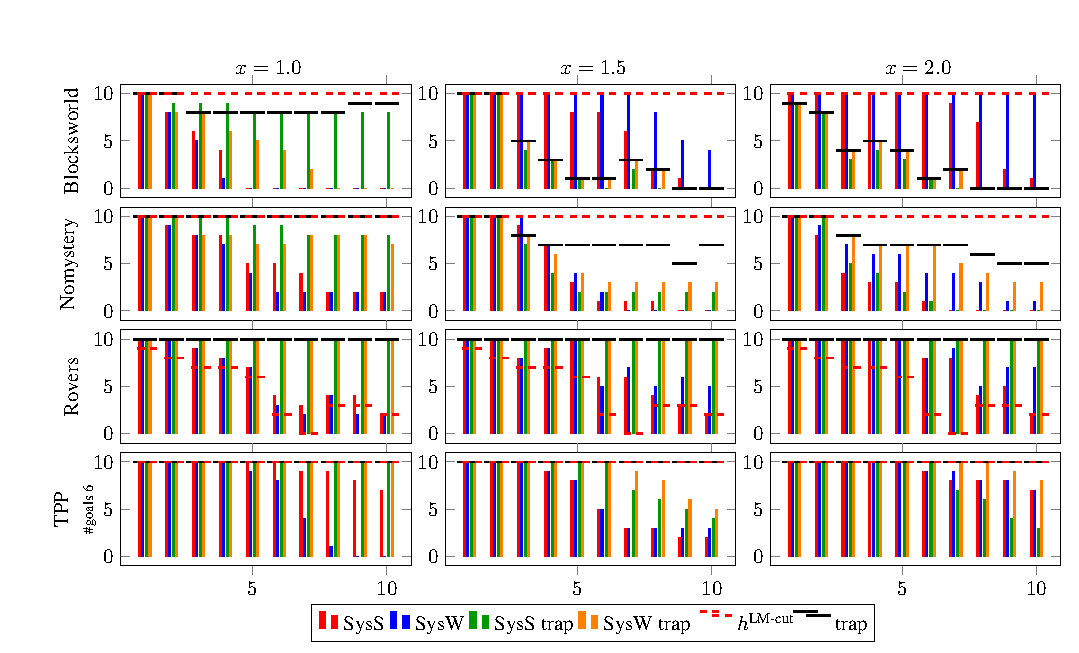
\includegraphics{data/action_set_properties/barchart/barchart.pdf}
%% \vspace{-0.6cm}
%% \caption{Coverage results on IPC benchmarks extended with action-set properties.}
%% \label{fig:barcharts}
%% \vspace{-0.2cm}
%% \end{figure*}

%% To evaluate the use of our framework with more complex plan
%% properties, beyond goal facts, we experimented with the compilation of
%% action-set properties as per Section~\ref{compilation}. We selected
%% four IPC domains for extension with action-set properties, namely
%% NoMystery, Rovers, and TPP as considered in resource-constrained
%% planning \cite{nakhost:etal:icaps-12}, where minimum resource
%% requirements are known as per available problem generators; plus the
%% Blocksworld as an intuitively rather differently structured domain. In
%% all four domains, we use discrete resource consumption encoded into
%% the STRIPS model, enabling the use of trap
%% learning \cite{steinmetz:hoffmann:ijcai-17} which turns out to be
%% highly beneficial here.

%% In Blocksworld, we include two gripper hands and the action-set
%% properties ask whether a given gripper is used to pick up a given
%% block, or to stack a given pair of blocks. In NoMystery, the
%% properties are as in our illustrative example
%% (Section~\ref{illustrative-example}). In Rovers, the properties ask
%% whether a given rover or camera is used for a given observation. In
%% TPP, they ask whether given road segments are used, and whether given
%% goods are bought at given markets. In all cases, we vary the number of
%% action-set properties between 1 and 10. We fix the original goal facts
%% as hard goals, and we set the available resources to $x \in \{1.0,1.5,
%% 2.0\}$ times the minimum needed to allow for costlier plans satisfying
%% some of the properties.

%% We created benchmark tasks with size parameters around the borderline
%% of computational feasibility for our analyses, given our time/memory
%% limits. In Blocksworld, we used 5 -- 8 blocks; in NoMystery, our tasks
%% have 2 trucks, 6 locations, and 4 -- 7 packages; in Rovers, they have
%% 2 rovers, 5 waypoints, and 4 -- 7 science objectives; in TPP, we use 5
%% markets, 1 depot, and 4 -- 7 goods. In all domains, we vary the number
%% of goal facts (and associated objects) between 4 and 7. We create 10
%% base instances for each size-parameter setting, which are then
%% modified for our experiments with different initial resource levels,
%% and action-set properties to be considered.
%% %
%% %% \begin{enumerate}
%% %% \item The resource constrained \textit{rovers} domain. Problems were generated with 2 rovers, 5 waypoints. Action properties are to use a specific rover for a sample or an observation, or to use a specific camera for an observation. 
%% %% \item The \textit{blocksworld} domain with 2 grippers, modified such that picking up or unstacking a block costs high or low energy depending upon which gripper is used. Problems were generated scaling from 3 to 10 blocks. Action properties are to use a specific gripper to pick up a specific block, or to use any gripper to stack a specific pair of blocks at any point in the plan.
%% %% \item The resource constrained \textit{TPP} domain. Problems were generated with 5 markets and 1 depot. Properties are to use or not use particular road segments, and preferred markets for goods.
%% %% \item The resource constrained \textit{nomystery} domain, described in the example. Problems were generated with 6 locations and 2 trucks.
%% %% \end{enumerate}

%% To have some comparison measure for performance, again we use
%% classical-planning reference points, based on \astar\ with \hlmcut,
%% and on search with trap learning, respectively. We now run these
%% reference points on tasks where all (original goal facts plus)
%% action-set properties are hard goals. These tasks may be solvable (in
%% which case \astar\ with \hlmcut\ tends to be better) or unsolvable (in
%% which case trap learning tends to be better). The configurations of
%% our own algorithm are SysS and SysW as before, now with vs.\ without
%% trap learning (and transfer).

%% Figure~\ref{fig:barcharts} shows the coverage data. To give an
%% overview, we show one row per domain, fixing the number of hard goals
%% at the feasibility borderline. Smaller numbers of goal facts tend to
%% be quite easy, larger ones mostly infeasible, with variance depending
%% on the domain and algorithm.
%% Appendix~\ref{data-action-set-properties} gives complete data for each
%% of the four domains.

%% In Blocksworld, the best of our techniques are moderately competitive
%% with the \hlmcut\ reference point (which starts to lose coverage when
%% one more block is added). They match the performance of the other
%% reference point for $x=1.0$, and surpass it for larger $x$ where trap
%% learning incurs a prohibitive overhead. NoMystery is the most
%% problematic domain in terms of performance, with all our techniques
%% lagging far behind the two reference points. In Rovers,
%% though, \astar\ with \hlmcut\ is much less effective than our
%% techniques, which match the full coverage of the trap-learning
%% reference point. TPP is similar to Blocksworld in that our techniques
%% are moderately competitive with the reference points. 
%% %\joerg{statement where coverage for these starts to go down} 
%% Trap learning is highly
%% beneficial in all cases except Blocksworld with $x>1.0$. Overall, it
%% seems fair to say that our action-set property dependency analysis is
%% not exceedingly infeasible compared to related classical planning
%% problems.


%% \fi

%%%% END IJCAI SUPPLEMENTARY MATERIAL VERSION
%%%%%%%%%%%%%%%%%%%%%%%%%%%%%%%%%%%%%%%%%%%%%%%%%%%%%%%%%%%%%%%%%%%%
%%%%%%%%%%%%%%%%%%%%%%%%%%%%%%%%%%%%%%%%%%%%%%%%%%%%%%%%%%%%%%%%%%%%
%%%%%%%%%%%%%%%%%%%%%%%%%%%%%%%%%%%%%%%%%%%%%%%%%%%%%%%%%%%%%%%%%%%%

